\subsection{正则局部环的定义}

令 A 为诺特局部环。设 \((x_{i})_{i\in I}\) 是 \(m_{A}\) 中元素的一个族。根据 II, § 3, n° 2 的命题 4 的推论 2，假设族 \((x_{i})_{i\in I}\) 生成 A 的理想 \(m_{A}\)，或假设 \(x_{i}\) 模 \(m_{A}^{2}\) 的类生成 \(\kappa_{A}\) -向量空间 \(m_{A}/m_{A}^{2}\)，两者是等价的；若如此，由 § 3, n° 2 的推论，有 dim(A) ≤ Card(I)。因而有不等式

\[
\dim (A) \leqslant [ m _ {A} / m _ {A} ^ {2}: \kappa_ {A} ] \leqslant \operatorname{Card} (I)\tag{1}
\]

对于每个族 \((x_{i})_{i\in I}\)，若其生成 A 的理想 \(m_{A}\)，则都有此不等式。

定义 1. --- 如果有 \(\dim(A) = [m_A/m_A^2:\kappa_A]\)，则称诺特局部环 A 为正则的。A 的坐标系是指 \(m_A\) 中的每个元素族，其模 \(m_A^2\) 的类构成 \(\kappa_A\)-向量空间 \(m_A/m_A^2\) 的一个基。

因此，正则诺特局部环 A 的一个坐标系是有限族 \((x_{i})_{i\in I}\)，它生成 A 的理想 \(m_{A}\)，并满足 \(\text{Card}(I) = \dim(A)\)。反之，若诺特局部环 A 的理想 \(m_{A}\) 由 d 个元素生成，且 \(d \leqslant \dim(A)\)，则环 A 是正则的。

例子。--- 1) 维数为 0（分别为 1）的正则诺特局部环是域（分别为离散赋值环）（VI, § 3, n° 6, 命题 9 以及下文定理 1 的推论 1）。设 A 是离散赋值环；则 m \(_{A}\) 中的元素 t 是一致化元，当且仅当 \{t\} 是 A 的一个坐标系。

\begin{enumerate}
\def\labelenumi{\arabic{enumi})}
\setcounter{enumi}{1}
\tightlist
\item
  令 \(k\) 为域，令 \(n\) 为正整数。形式幂级数环 \(k[[X_1, ..., X_n]]\) 是维数为 \(n\) 的正则诺特局部环（§ 3, n° 4, 命题 8 的推论 3）。令 \(F_1, ..., F_n\) 为 \(k[[X_1, ..., X_n]]\) 中无常数项的形式幂级数；序列 \((F_1, ..., F_n)\) 成为 \(k[[X_1, ..., X_n]]\) 的一个坐标系的充要条件是矩阵 \(\left(\frac{\partial F_i}{\partial X_j}(0, ..., 0)\right)\) 可逆。
\end{enumerate}

更一般地，设 A 是维数为 \(r\) 的正则诺特局部环；则 \(A[[X_1, ..., X_n]]\) 是维数为 \(r + n\) 的正则诺特局部环。若 \((a_1, ..., a_r)\) 是 A 的一个坐标系，则 \((a_1, ..., a_r, X_1, ..., X_n)\) 是 \(A[[X_1, ..., X_n]]\) 的一个坐标系。

\begin{enumerate}
\def\labelenumi{\arabic{enumi})}
\setcounter{enumi}{2}
\tightlist
\item
  令 A 是维数为 \(r\) 的完备正则诺特局部环。受限形式幂级数环 A \(\{X_1, ..., X_n\}\) 是维数为 \(r + n\) 的正则诺特局部环（§ 3, n° 4, 注 1）。若 \((a_1, ..., a_r)\) 是 A 的一个坐标系，则 \((a_1, ..., a_r, X_1, ..., X_n)\) 是 A \(\{X_1, ..., X_n\}\) 的一个坐标系。
\end{enumerate}

* 4) 令 \(k\) 为完备非离散赋值域。\(n\) 元形式幂级数在 \(k^n\) 中 0 的某邻域内收敛时所成的环，是维数为 \(n\) 的正则诺特局部环 ( \(\S\) 3, n° 4, 注 2). *

\begin{enumerate}
\def\labelenumi{\arabic{enumi})}
\setcounter{enumi}{4}
\tightlist
\item
  令 \(k\) 为域，A 为有限型 \(k\)-代数且为整环，\(\mathfrak{m}\) 为 A 的极大理想。诺特局部环 \(\mathrm{A}_{\mathfrak{m}}\) 是正则的，当且仅当有 \(\dim(\mathrm{A}) = [\mathfrak{m}/\mathfrak{m}^{2}:\mathrm{A}/\mathfrak{m}]\)：事实上，有 \(\dim(\mathrm{A}_{\mathfrak{m}}) = \dim(\mathrm{A})\) ( \(\S 2\) , \(no. 4\) , 定理 3 的推论 2)，并且关于域 A/m 的向量空间 \(\mathfrak{m}/\mathfrak{m}^{2}\) 与 \(\mathrm{mA}_{\mathfrak{m}}/(\mathrm{mA}_{\mathfrak{m}})^{2}\) 同构（II, \(\S 3\) , \(no. 3\) , 命题 9）。特别地，若 \(k\) 代数闭，所述条件等价于 \(\dim(\mathrm{A}) = [\mathfrak{m}/\mathfrak{m}^{2}:k]\)（V, \(\S 3\) , \(no. 3\) , 命题 1）。
\end{enumerate}

* 6) 设 X 是完美域 \(k\) 上的代数簇。X 在点 \(x\) 处非奇异，当且仅当 X 在 \(x\) 处的局部环是正则的。*

* 7) 设 A 是正则诺特局部环。稍后将看到，对于 A 的每个素理想 p，诺特局部环 \(A_{p}\) 都是正则的。 *

命题 1.--- 设 A、B 是诺特局部环，\(\rho:A\to B\) 是一个局部同态，并使 B 成为平坦 A-模。设有 \(m_{B} = B \cdot \rho(m_{A})\)。则有 \(\dim(A) = \dim(B)\)，且 B 正则当且仅当 A 正则。

第一条断言由 § 3, no. 4 的命题 7 的推论 1 得出。由于 B 在 A 上平坦，可将 \(\mathfrak{m}_{\mathrm{B}}^{k} = \mathbf{B}.\rho (\mathfrak{m}_{\mathrm{A}}^{k})\) 认作 \(\mathbf{B}\otimes_{\mathbf{A}}\mathfrak{m}_{\mathbf{A}}^{k}\)，对于每个满足 \(k\geqslant 0\) 的整数，进而将 \(\mathfrak{m}_{\mathrm{B}} / \mathfrak{m}_{\mathrm{B}}^{2}\) 认作 \(\mathbf{B}\otimes_{\mathbf{A}}(\mathfrak{m}_{\mathrm{A}} / \mathfrak{m}_{\mathrm{A}}^{2})\)，或也可认作 \(\kappa_{\mathrm{B}}\otimes_{\kappa_{\mathrm{A}}}(\mathfrak{m}_{\mathrm{A}} / \mathfrak{m}_{\mathrm{A}}^{2})\)。因而有

\[
\left[ \mathfrak {m} _ {\mathrm{B}} / \mathfrak {m} _ {\mathrm{B}} ^ {2}: \kappa_ {\mathrm{B}} \right] = \left[ \mathfrak {m} _ {\mathrm{A}} / \mathfrak {m} _ {\mathrm{A}} ^ {2}: \kappa_ {\mathrm{A}} \right],\tag{2}
\]

命题立即由此得到。

推论。--- 诺特局部环 A 正则，当且仅当其完备化 \(\hat{A}\) 正则。

事实上，\(\hat{\mathbf{A}}\) 在 \(\mathbf{A}\) 上平坦，且有 \(\mathfrak{m}_{\hat{\mathbf{A}}} = \hat{\mathbf{A}}. \mathfrak{m}_{\mathbf{A}}\)（III, § 3, no. 4, 定理 3 以及 § 2, no. 12, 命题 16 的推论 2）。

\subsection{与正则局部环关联的分次环}

定理 1. --- 设 A 为诺特局部环。下列条件彼此等价：

\begin{enumerate}
\def\labelenumi{(\roman{enumi})}
\item
  A 是正则的。
\item
  理想 \(\mathfrak{m}_{\mathbf{A}}\) 由 A 的一个正割子集生成（§ 3, no. 2, 定义 1）。
\item
  理想 \(\mathfrak{m}_{\mathrm{A}}\) 由 A 的一个完全正割序列生成（A, X, p.~157, 定义 2）。
\item
  令 S 为 \(\kappa_{\mathbf{A}}\)-向量空间 \(\mathfrak{m}_{\mathbf{A}} / \mathfrak{m}_{\mathbf{A}}^{2}\) 的对称代数，并令 \(\operatorname{gr}(\mathbf{A}) = \bigoplus_{n \geqslant 0} \mathfrak{m}_{\mathbf{A}}^{n} / \mathfrak{m}_{\mathbf{A}}^{n+1}\) 为与 A 关联的分次环。S 的典范同态 \(\gamma\) 映到 \(\operatorname{gr}(\mathbf{A})\) 上是双射。
\item
  存在整数 \(r \geqslant 0\)，使得 \(H_{\mathbf{A},\mathfrak{m}_{\mathbf{A}}} = (1 - \mathrm{T})^{-r}\)，即 \(\mathfrak{m}_{\mathbf{A}} = 0\) 当 \(r = 0\) 时；并且等式 \([\mathfrak{m}_{\mathbf{A}}^{n}/\mathfrak{m}_{\mathbf{A}}^{n+1}:\kappa_{\mathbf{A}}] = \binom{n + r - 1}{r - 1}\) 对每个满足 \(n \geqslant 0\) 的整数成立（在 \(r > 0\) 时）。
\item
  我们有 \(\mathrm{H}_{\mathrm{A},\mathfrak{m}_{\mathrm{A}}} = (1 - \mathrm{T})^{-d}\)，其中 \(d = \dim (\mathrm{A})\)。
\end{enumerate}

如果这些条件成立，则 A 的每个坐标系都是 A 的一个完全正割序列。

\begin{enumerate}
\def\labelenumi{(\roman{enumi})}
\setcounter{enumi}{1}
\item
  \(\Rightarrow\) (i)：事实上，每个正割子集至多含有 dim(A) 个元素（ \(\S 3\) , no. 2, 定理 1）。
\item
  \(\Rightarrow\) (ii)：事实上，每个完全正割序列都是正割的（§ 3, no. 2, 命题 3 的推论）。
\end{enumerate}

\((\mathrm{iv}) \Rightarrow (\mathrm{iii}) : \text{设 } (x_1, ..., x_r)\) 是 \(\mathfrak{m}_{\mathbf{A}}\) 中元素的一个序列，其模 \(\mathfrak{m}_{\mathbf{A}}^2\) 的类形成 \((\xi_1, ..., \xi_r)\)，后者是 \(\mathfrak{m}_{\mathbf{A}} / \mathfrak{m}_{\mathbf{A}}^2\) 关于域 \(\kappa_{\mathbf{A}}\) 的一个基。若性质 (iv) 成立，则 \(\operatorname{gr}(\mathbf{A})\) 是多项式代数 \(\kappa_{\mathbf{A}}[\xi_1, ..., \xi_r]\)，且序列 \((x_1, ..., x_r)\) 是完全正割序列（A, X, p.~160, 定理 1）。这也证明了定理 1 的最后一个断言。

\begin{enumerate}
\def\labelenumi{(\roman{enumi})}
\tightlist
\item
  \(\Rightarrow\) (iv)：置 \(r = [\mathfrak{m}_{\mathbf{A}} / \mathfrak{m}_{\mathbf{A}}^{2}:\kappa_{\mathbf{A}}]\)。根据 § 4, no. 2 的公式 (6)，分次向量空间 S 关于域 \(\kappa_{\mathbf{A}}\) 的庞加莱级数等于
\end{enumerate}

\[
\mathrm{P} _ {\mathrm{S}} = \sum_ {n \geqslant 0} \left[ \mathrm{S} ^ {n} (\mathfrak {m} _ {\mathrm{A}} / \mathfrak {m} _ {\mathrm{A}} ^ {2}): \kappa_ {\mathrm{A}} \right] \mathrm{T} ^ {n} = (1 - \mathrm{T}) ^ {- r}.
\]

设典范同态 \(\gamma: S \to \mathrm{gr}(A)\) 不是双射。由于 \(\gamma\) 是满射，S 中存在齐次元素 \(u\)，它属于 \(S\)，次数为 \(d > 0\)，且被 \(\gamma\) 消去。于是有

\[
\begin{array}{r l} \mathrm {H_ {A,m_ {A}}} = & \mathrm {P_ {S}} - \symrm {P_ {Ker(\gamma)}} \leqslant \mathrm {P_ {S}} - \mathrm {P_ {uS}} = (1 - \mathrm{T} ^ {d}) / (1 - \mathrm{T}) ^ {r} = \\ & = (1 + \mathrm{T} + \dots + \mathrm{T} ^ {d - 1}) / (1 - \mathrm{T}) ^ {r - 1}. \end{array}
\]

根据 § 4, no. 4 的定理 3 和 § 4, no. 1 的引理 2，因而有 dim(A) \textless{} r，且 A 不是正则的。

最后证明条件 (iv) 至 (vi) 的等价性。现在，(iv) 意味着我们有 \(\mathrm{H}_{\mathrm{A},\mathfrak{m}_{\mathrm{A}}}=(1-\mathrm{T})^{-s}\)，其中 \(s=[\mathfrak{m}_{\mathrm{A}}/\mathfrak{m}_{\mathrm{A}}^{2}:\kappa_{\mathrm{A}}]\)。因此，条件 (iv)、(v)、(vi) 意味着我们有 \(\mathrm{H}_{\mathrm{A},\mathfrak{m}_{\mathrm{A}}}=(1-\mathrm{T})^{-m}\)，其中相应地 \(m=[\mathfrak{m}_{\mathrm{A}}/\mathfrak{m}_{\mathrm{A}}^{2}:\kappa_{\mathrm{A}}]\)、\(m\geqslant0\)、\(m=\dim(\mathrm{A})\)。但是，若有 \(\mathrm{H}_{\mathrm{A},\mathfrak{m}_{\mathrm{A}}}=(1-\mathrm{T})^{-m}\)，则根据 §4, no. 4, 定理 3，有 \(\dim(\mathrm{A})=m\)，并且有 \([\mathfrak{m}_{\mathrm{A}}/\mathfrak{m}_{\mathrm{A}}^{2}:\kappa_{\mathrm{A}}]=m\)（因为 \((1-\mathrm{T})^{-m}=1+m\mathrm{T}+\cdots\)）。条件 (iv) 与 (vi) 的等价性立即得到。

推论 1. --- 每个正则诺特局部环都是整闭的，因而特别是整环。

假设 A 正则。则 gr(A) 同构于域上有限多个不定元的多项式代数（定理 1, (iv)）。因此，gr(A) 是诺特整闭环（V, § 1, no. 3, 命题 13 的推论 3），从而 A 是整闭的（V, § 1, no. 4, 命题 15）。

我们将在后面的章节中看到，每个正则诺特局部环都是唯一分解环。

推论 2.--- 设 A、B 是诺特局部环，σ 是从 B 到 A 的局部同态。设 A 正则且 B 完备。σ 为双射的充要条件是：σ 将 κ \(_{B}\) 双射到 κ \(_{A}\)，并将 m \(_{B}\) /m \(_{B}^{2}\) 双射到 m \(_{A}\) /m \(_{A}^{2}\)。

所述条件显然是必要的。

反之，假设 \(\sigma\) 将 \(\mathrm{gr}_{0}(\mathbf{B})\) 同构到 \(\mathrm{gr}_{0}(\mathbf{A})\)，并将 \(\mathrm{gr}_{1}(\mathbf{B})\) 同构到 \(\mathrm{gr}_{1}(\mathbf{A})\)。由于环 \(\mathrm{gr}(\mathbf{B})\) 由 \(\mathrm{gr}_{0}(\mathbf{B}) \cup \mathrm{gr}_{1}(\mathbf{B})\) 生成，而 \(\mathrm{gr}(\mathbf{A})\) 是 \(\mathrm{gr}_{1}(\mathbf{A})\) 作为 \(\mathrm{gr}_{0}(\mathbf{A})\) 上向量空间的对称代数，故同态 \(\mathrm{gr}(\sigma)\) 是双射。因此，\(\sigma\) 是双射（III, § 2, no. 8, 定理 1 的推论 3）。

推论 3. --- 设 \(k\) 为域，A 为局部诺特 \(k\)-代数，且其剩余域等于 \(k\)。A 正则的充要条件是：其完备化 \(\hat{A}\) 同构于一个 \(k\)-代数，该代数由形式级数 \(k[[X_1, ..., X_n]]\) 构成。

这由定理 1 中 (i) 与 (iv) 的等价性以及 III, § 2, no. 9 的命题 11 得出。

\subsection{正则局部环的商环}

命题 2. --- 设 A 是诺特局部环，\(\boldsymbol{x} = (x_1, ..., x_r)\) 是 \(\mathfrak{m}_{\mathrm{A}}\) 中元素的一个序列，且 \(\mathfrak{x}\) 是由 \(\boldsymbol{x}\) 生成的理想。下列条件等价：

\begin{enumerate}
\def\labelenumi{(\roman{enumi})}
\item
  A 是正则的，且 x 是 A 的一个坐标系的一部分；
\item
  环 A/x 是正则的，且 x 是 A 的一个正割序列；
\item
  环 A/x 是正则的，且 x 是 A 的一个完全正割序列。
\end{enumerate}

此外，在这些条件成立时，x 是 A 的一个素理想。

\begin{enumerate}
\def\labelenumi{(\roman{enumi})}
\setcounter{enumi}{2}
\item
  \(\Rightarrow\) (ii)：这由 § 3, no. 2 的命题 3 的推论得出。
\item
  \(\Rightarrow\) (i)：设 \(x\) 是 A 的一个正割序列，且诺特局部环 A/\(x\) 是正则的。设 \((x_{r+1}, ..., x_d)\) 是 A 中元素的一个序列，其模 \(x\) 的类构成 A/\(x\) 的一个坐标系。则序列 \((x_1, ..., x_d)\) 生成 A 的理想 \(m_A\)，且有
\end{enumerate}

\[
\dim (\mathrm{A}) = r + \dim (\mathrm{A} / \mathrm{x}) = r + (d - r) = d.
\]

因此，A 是正则的，且 \((x_{1},\ldots,x_{d})\) 是 A 的一个坐标系。

\begin{enumerate}
\def\labelenumi{(\roman{enumi})}
\tightlist
\item
  \(\Rightarrow\) (iii)：若条件 (i) 成立，则序列 \(x\) 是完全正割的（no. 2, 定理 1），从而根据 § 3, no. 2 的命题 3 的推论，它是正割的。因此有
\end{enumerate}

\[
\dim (\mathrm{A} / \mathfrak {x}) = \dim (\mathrm{A}) - r;\tag{3}
\]

此外，\(x_{1},\ldots,x_{r}\) 模 \(\mathfrak{m}_{\mathbf{A}}^{2}\) 的类在域 \(\kappa_{\mathbf{A}}\) 上线性无关，因此有

\[
\left[ \mathfrak {m} _ {\mathrm{A}} / (\mathfrak {m} _ {\mathrm{A}} ^ {2} + x): \kappa_ {\mathrm{A}} \right] = \left[ \mathfrak {m} _ {\mathrm{A}} / \mathfrak {m} _ {\mathrm{A}} ^ {2}: \kappa_ {\mathrm{A}} \right] - r.\tag{4}
\]

公式 (3) 和 (4) 表明 A/x 是正则的。

根据第 2 号的定理 1 的推论 1，每个正则诺特局部环都是整环。因此，如果 A/x 正则，则 x 是素理想。

推论 1. --- 设 A 是诺特局部环，且 t 是 \(\mathfrak{m}_{\mathrm{A}}\) 中的元素。下列条件等价：

\begin{enumerate}
\def\labelenumi{(\roman{enumi})}
\item
  A 是正则的，且 t 不属于 \(m_{A}^{2}\)；
\item
  A/tA 是正则的，且 \(\dim(\mathrm{A}/t\mathrm{A}) < \dim(\mathrm{A})\)；
\item
  A/tA 是正则的，且 t 不是 A 中的零因子。
\end{enumerate}

推论 2. --- 设 A 是正则诺特局部环，q 是 A 的一个理想。A/q 正则，当且仅当 q 由 A 的一个坐标系的某个子集生成。

充分性由命题 2 得出。

假设 A/q 正则，令 \(x = (x_{1}, \ldots, x_{r})\) 为 q 中元素的一个序列，其模 \(m_{A}^{2}\) 的类构成 \((\mathfrak{q} + \mathfrak{m}_{\mathrm{A}}^{2})/\mathfrak{m}_{\mathrm{A}}^{2}\) 关于域 \(\kappa_{A}\) 的一个基。令 x 为 A 中由 x 生成的理想。因此有 \(x \subset q\)，且 x 是 A 的一个坐标系的一部分，所以诺特局部环 A/x 是正则的（命题 2）；此外，向量空间 \(\mathfrak{m}_{\mathrm{A}}/(\mathfrak{q} + \mathfrak{m}_{\mathrm{A}}^{2})\) 与 \(\mathfrak{m}_{\mathrm{A}}/(\mathfrak{x} + \mathfrak{m}_{\mathrm{A}}^{2})\) 关于 \(\kappa_{A}\) 具有相同维数。因此，正则诺特局部环 A/q 和 A/x 具有相同维数。由于理想 q 和 x 都是素理想，且有 \(x \subset q\)，最后得到 q = x。

例。--- 设 \(k\) 为域，\(\mathbf{A} = k[[\mathbf{X}_1, ..., \mathbf{X}_n]]\)，\(\mathfrak{q}\) 是 \(\mathbf{A}\) 的理想且不同于 \(\mathbf{A}\)。\(\mathbf{A}/\mathfrak{q}\) 正则的充要条件是：存在整数 \(r \geqslant 0\) 以及元素 \(\mathbf{F}_1, ..., \mathbf{F}_r\)，这些元素属于 \(\mathbf{A}\)，生成 \(\mathfrak{q}\)，并且矩阵 \(\left(\frac{\partial\mathbf{F}_i}{\partial\mathbf{X}_j}(0, ..., 0)\right)\) 的秩为 \(r\)（“雅可比判据”）。于是 \(\dim(\mathbf{A}/\mathfrak{q}) = n - r\)。

注。--- 设 A 是正则诺特局部环，且 \(q \subset m_{A}\) 是 A 的一个理想，使得 A/q 正则。设 \((x_{1}, \ldots, x_{r})\) 是 q 中元素的一个序列，其模 \(m_{A}^{2}\) 的类生成向量空间 \((\mathfrak{q} + \mathfrak{m}_{\mathrm{A}}^{2}) / \mathfrak{m}_{\mathrm{A}}^{2}\)（关于域 \(\kappa_{A}\)）。命题 2 的推论 2 的证明表明，A 的理想 q 由 \((x_{1}, \ldots, x_{r})\) 生成。

\subsection{艾森斯坦多项式}

定义 2. --- 设 A 是环，p 是 A 的素理想，P 是 A{[}T{]} 中的多项式。如果 P 满足以下条件，则称 P 是关于 p 的艾森斯坦多项式：

\begin{enumerate}
\def\labelenumi{\alph{enumi})}
\item
  P 是次数 \(d \geqslant 1\) 的首一多项式；
\item
  有 \(\mathrm{P(T)}\equiv \mathrm{T}^d\bmod \mathfrak{pA}[\mathrm{T}];\)
\item
  有 \(\mathbf{P}(0)\notin \mathfrak{p}^2\)
\end{enumerate}

换言之，关于 p 的艾森斯坦多项式是形如 \(\mathbf{P}(\mathbf{T}) = \mathbf{T}^{d} + \sum_{i=1}^{d} a_{i} \mathbf{T}^{d-i}\) 的多项式，其中 \(d \geqslant 1\)，\(a_{1}, \ldots, a_{d-1}\) 属于 p，且 \(a_{d}\) 属于 \(p - p^{2}\)。

称 P 是关于 \(pA_{p}\) 的艾森斯坦多项式，当且仅当 P 在多项式环 \(A_{p}[T]\) 中的典范像是关于理想 \(pA_{p}\) 的艾森斯坦多项式；这也意味着 P 是关于 p 的艾森斯坦多项式，并且还满足下述比 c) 更强的条件：

\(c^{\prime})\) A 中每个元素 \(a\)，只要 \(a\mathbf{P}(0)\in\mathfrak{p}^{2}\)，就属于 \(\mathfrak{p}\)。

命题 3. --- 设 A 是环，p 是 A 的素理想，P ∈ A{[}T{]} 是关于 p 的艾森斯坦多项式。

\begin{enumerate}
\def\labelenumi{\alph{enumi})}
\item
  不存在形如 \(P = P_{1}P_{2}\) 的分解，其中 \(P_{1}\) 和 \(P_{2}\) 是 A{[}T{]} 中不同于 1 的两个首一多项式。
\item
  假设 A 整闭，分式域为 K。则 P 在 K[T] 中不可约。
\end{enumerate}

令 \(\varphi\) 为从 A 到 A/p 的分式域 \(k\) 的典范同态，并令 \(\varphi':\mathrm{A}[\mathrm{T}]\to k[\mathrm{T}]\) 为 \(\varphi\) 的延拓，使得 \(\varphi'(\mathrm{T})=\mathrm{T}\)。假设 \(\mathbf{P}=\mathbf{P}_{1}\mathbf{P}_{2}\)，其中 \(\mathbf{P}_{1}\) 和 \(\mathbf{P}_{2}\) 是 A{[}T{]} 中不同于 1 的两个首一多项式。于是有 \(\mathrm{T}^{d}=\varphi'(\mathbf{P}_{1})\varphi'(\mathbf{P}_{2})\)，且等式成立于 \(k[\mathrm{T}]\) 中，其中 \(d\) 为 P 的次数。若 \(d_{i}\) 是 \(\mathbf{P}_{i}\) 的次数，则有 \(\varphi'(\mathbf{P}_{i})=\mathrm{T}^{d_{i}}\)，即 \(\mathbf{P}_{i}(\mathrm{T})\equiv\mathrm{T}^{d_{i}}\text{ mod. pA[T]}\)，特别地，\(\mathbf{P}_{i}(0)\in\mathfrak{p}\)。但是 \(\mathrm{P}(0)=\mathrm{P}_{1}(0).\mathrm{P}_{2}(0)\) 属于 \(\mathfrak{p}^{2}\)，这与假设矛盾。这证明了 \(a\)。

断言 \(b)\) 由 \(a)\) 以及 V, § 1, no. 3 的命题 11 得出。

设 A 是诺特局部环，且 \(P_{1}, \ldots, P_{r}\) 是 A{[}T{]} 中次数为 \(\geqslant 2\) 的首一多项式。令 q 为 A{[}T \(_{1}\) , \ldots, T \(_{r}\) {]} 的理想，它由 \(\mathrm{P}_{1}(\mathrm{T}_{1}), \ldots, \mathrm{P}_{r}(\mathrm{T}_{r})\) 生成；令 B 为商 A-代数 A{[}T \(_{1}\) , \ldots, T \(_{r}\) {]}/q。对于 \(1 \leqslant i \leqslant r\)，记 \(d_{i}\) 为 \(P_{i}, t_{i}\) 的相关数据：前者表示 P＿i 的次数，后者表示 T \(_{i}\) 模 q 的类；并记 \(\gamma_{i}\) 为 \(c_{i} = \mathrm{P}_{i}(0)\) 模 \(m_{A}^{2}\) 的类。假设有 \(\mathrm{P}_{i}(\mathrm{T}) \equiv \mathrm{T}^{d_{i}} \mod \mathrm{m}_{\mathrm{A}}\mathrm{A}[\mathrm{T}]\)，这对 \(1 \leqslant i \leqslant r\) 成立。

命题 4. --- a) 环 B 是局部诺特环，其极大理想为

\[
\mathfrak {m} _ {\mathrm{B}} = \mathbf {B m} _ {\mathrm{A}} + \sum_ {i = 1} ^ {r} \mathbf {B t} _ {i}.
\]

有 \(\dim(\mathbf{A}) = \dim(\mathbf{B})\)，且 \([\kappa_{\mathbf{B}}: \kappa_{\mathbf{A}}] = 1\)。单项式 \(t_1^{\alpha(1)} \ldots t_r^{\alpha(r)}\)，其中 \(0 \leqslant \alpha(i) < d_i\)，且 \(1 \leqslant i \leqslant r\)，构成 A-模 B 的一个基。

\begin{enumerate}
\def\labelenumi{\alph{enumi})}
\setcounter{enumi}{1}
\item
  令 \(\lambda\) 为从 \(\mathfrak{m}_{\mathbf{A}} / \mathfrak{m}_{\mathbf{A}}^{2}\) 到 \(\mathfrak{m}_{\mathbf{B}} / \mathfrak{m}_{\mathbf{B}}^{2}\) 的典范同态。则 \(\lambda\) 的核是一个 \(\kappa_{\mathbf{A}}\)-向量空间，由 \(\gamma_{1}, \ldots, \gamma_{r}\) 生成。元素 \(t_{1}, \ldots, t_{r}\) 的类关于 \(\kappa_{\mathbf{A}}\) 构成 \(\lambda\) 的余核的一个基。
\item
  B 正则的充要条件是 A 正则，且 \(\gamma_{1},\ldots,\gamma_{r}\) 在 \(\kappa_{\mathbf{A}}\)-向量空间 \(\mathfrak{m}_{\mathbf{A}}/\mathfrak{m}_{\mathbf{A}}^{2}\) 中线性无关。
\end{enumerate}

A-代数 B 同构于张量积 \(B_{1} \otimes_{A} \cdots \otimes_{A} B_{r}\)，其中 \(B_{i} = A[T]/(P_{i})\)，\(1 \leqslant i \leqslant r\)。因此，单项式 \(t_{1}^{\alpha(1)} \ldots t_{r}^{\alpha(r)}\)，其中 \(0 \leqslant \alpha(i) < d_{i}\)，且 \(1 \leqslant i \leqslant r\)，构成 A-模 B 的一个基。特别地，B 在 A 上整，故根据 § 2, no. 3 的定理 1，A 与 B 具有相同维数。

根据 IV, § 2, no. 5 的命题 9 的推论 3，环 B 是诺特的，并且 B 的每个极大理想都包含 B.m\_A。此外，由于对 P\_1, \ldots P\_r 所作的假设以及关系 P\_i(t\_i) = 0，有 t\_i\^{}\{d\_i\} ∈ B.m\_A（1 ≤ i ≤ r）。因此 B 的每个极大理想都包含 t\_1, \ldots, t\_r，因而也包含理想 q' = B.m\_A + Bt\_1 + \ldots{} + Bt\_r。现在有 m\_A = A ∩ q' 且 B = A + q'，故 B/q' 同构于 A/m\_A，而 q' 是 B 的一个极大理想；所以 B 是局部的，且有 {[}κ\_B : κ\_A{]} = 1。这证明了 a)。

置 \(\mathfrak{r} = \mathfrak{m}_{A}^{2} + \sum_{i=1}^{r} A c_i\)，令 \(\varphi\) 为从 \((A/\mathfrak{m}_{A}^{2})[T_1, ..., T_r]\) 到 \(B/\mathfrak{m}_{B}^{2}\) 的典范同态。由于有 \(m_B = B.m_A + \sum_{i=1}^{r} B t_i\)，其核记为 \(n\)；关于 \(\varphi\)，该核由多项式的类 \(\overline{P}_i(T_i)\) 生成，其中多项式为 \(P_i(T_i)\)，并按模 \(\mathfrak{m}_{A}^{2}.A[T_1, ..., T_r]\) 取类；还由单项式 \(T_i T_j\) 和 \(x T_i\) 生成，其中 \(1 \leqslant i, j \leqslant r\)，且 \(x\) 属于 \(m_A/m_A^2\)。根据对 \(P_i\) 所作的假设，即 \(P_i(T) \equiv T^{d_i} \mod. m_A.A[T]\)，可在上述描述中将 \(\overline{P}_i(T_i)\) 替换为 \(\gamma_i\)，而这个描述涉及 \(n\)；因此，环 \(B/m_B^2\) 同构于 \(A/\mathfrak{r}\) \([T_{1}, ..., T_{r}]\) 关于分次理想的商，该理想由单项式 \(T_{i}T_{j}\) 和 \(xT_{i}\) 生成，其中 \(x\) 属于 \(m_A/\mathfrak{r}\)。记 \(\tau_{i}\) 为 \(t_{i}\) 模 \(m_{B}^{2}\) 的类；于是有

\[
\mathrm{B} / \mathfrak {m} _ {\mathrm{B}} ^ {2} = (\mathrm{A} / \mathfrak {r}) \oplus \kappa_ {\mathrm{A}} \tau_ {1} \oplus \dots \oplus \kappa_ {\mathrm{A}} \tau_ {r},\tag{5}
\]

从而

\[
\mathfrak {m} _ {\mathrm{B}} / \mathfrak {m} _ {\mathrm{B}} ^ {2} = (\mathfrak {m} _ {\mathrm{A}} / \mathfrak {r}) \oplus \kappa_ {\mathrm{A}} \tau_ {1} \oplus \dots \oplus \kappa_ {\mathrm{A}} \tau_ {r}.\tag{6}
\]

断言 b) 立即由此得到。

根据公式 (6) 及关系 \([\kappa_{\mathrm{B}}:\kappa_{\mathrm{A}}] = 1\)，有

\[
\left[ \mathfrak {m} _ {\mathrm{B}} / \mathfrak {m} _ {\mathrm{B}} ^ {2}: \kappa_ {\mathrm{B}} \right] = \left[ \mathfrak {m} _ {\mathrm{A}} / \mathfrak {m} _ {\mathrm{A}} ^ {2}: \kappa_ {\mathrm{A}} \right] + \left\{r - \left[ \mathfrak {r} / \mathfrak {m} _ {\mathrm{A}} ^ {2}: \kappa_ {\mathrm{A}} \right] \right\}.\tag{7}
\]

现在，\(\kappa_{\mathrm{A}}\)-向量空间 \(\mathfrak{r}/\mathfrak{m}_{\mathrm{A}}^{2}\) 由 \(\gamma_{1}, \ldots, \gamma_{r}\) 生成，且有

\[
\dim (\mathbf {B}) = \dim (\mathbf {A}) \leqslant [ \mathfrak {m} _ {\mathbf {A}} / \mathfrak {m} _ {\mathbf {A}} ^ {2}: \kappa_ {\mathbf {A}} ].\tag{8}
\]

断言 (c) 立即由公式 (7) 和 (8) 得出。

推论。--- 设 A 是正则诺特局部环，且 P ∈ A{[}T{]} 是关于 m\_A 的艾森斯坦多项式。环 B = A{[}T{]}/(P) 是与 A 同维数的正则诺特局部环，且有 {[}κ\_A : κ\_B{]} = 1。最后，有 m\_B = B.m\_A + Bt，其中 t 是 T 模 (P) 的类。

P 次数至少为 2 的情形由取 r = 1 应用命题 4 得出；当 P 次数为 1，即形如 T - c 且 \(c \in m_{A}\) 时，推论立即得到。

命题 5. --- 设 A 是整环，分式域为 K，L 是 K 的有限代数扩张。记 B 为 L 中 A 的整闭包，p 为 A 的一个素理想。

假设局部环 \(\mathbf{A}_{\mathfrak{p}}\) 是诺特且正则的；设 \(t\) 是 \(\mathbf{L}\) 中的元素，使得 \(\mathbf{L} = \mathbf{K}(t)\)，并假设在 \(\mathbf{A}[\mathbf{T}]\) 中存在元素 \(\mathbf{P}\)，它是关于 \(\mathfrak{p}\mathbf{A}_{\mathfrak{p}}\) 的艾森斯坦多项式，且 \(t\) 是其根。

\begin{enumerate}
\def\labelenumi{\alph{enumi})}
\item
  B 中存在唯一一个位于 p 之上的素理想 q。
\item
  局部环 \(\mathbf{B}_{\mathfrak{q}}\) 是诺特且正则的，并且与 \(\mathbf{A}_{\mathfrak{p}}\) 具有相同维数。
\item
  我们有 \(\mathbf{B}_{\mathfrak{q}} = \mathrm{A}_{\mathfrak{p}}[t]\)。
\item
  从 A/p 到 B/q 的典范同态在这些环的分式域之间诱导出一个同构。
\end{enumerate}

置 \(C = A_{p}[t]\)，记 \(d\) 为 P 的次数。将命题 3 应用于环 \(A_{p}\)，可知艾森斯坦多项式 P 在 K{[}T{]} 中不可约，且 \((1, t, ..., t^{d-1})\) 是 L 关于 K 的一个基，因而也是 C 关于 \(A_{p}\) 的一个基。由于 P 是首一的，从 \(A_{p}[T]\) 到 C 的典范同态的核等于 (P)。根据上面的命题 4 的推论，C 是与 \(A_{p}\) 具有相同维数的正则诺特局部环，C 的极大理想 \(m_{C}\) 由 \(p \cup \{t\}\) 生成，且域 \(\kappa_{C}\) 是 A/p 的分式域的平凡扩张。要证明命题 5，只需证明 B 上存在唯一一个位于 p 之上的素理想 q，并且有 \(C = B_{q}\)。

置 \(S = A - p\)。我们知道（V, § 1, no. 5, 命题 16），其整闭包

\(A_{p}\) 在 L 中等于 \(S^{-1}B\)。此外，t 在 \(A_{p}\) 上整，环 \(C = A_{p}[t]\) 是正则诺特局部环，因而是整闭的（no. 2, 定理 1 的推论 1）。所以有 \(C = S^{-1}B\)。因此，环 \(S^{-1}B\) 是局部的并且只有一个极大理想。根据 V, § 2, no. 1 的命题 1，\(S^{-1}B\) 在 \(pA_{p}\) 之上有唯一的素理想，所以 B 在 p 之上有唯一的素理想 q（同上，引理 1），并且有 \(B_{q} = S^{-1}B = C\)。

推论。--- 假设 \(A_{p}\) 是离散赋值环。则 \(B_{q}\) 是离散赋值环，t 是 \(B_{q}\) 的一致化元，且有

\[
f (\mathrm{B} _ {\mathfrak {q}} / \mathrm{A} _ {\mathfrak {p}}) = 1, e (\mathrm{B} _ {\mathfrak {q}} / \mathrm{A} _ {\mathfrak {p}}) = [ \mathrm{L}: \mathrm{K} ]\tag{9}
\]

(VI, § 8, no. 1).

事实上，离散赋值环正是维数为 1 的正则诺特局部环；置 \(d = [\mathrm{L}:\mathrm{K}]\)，有 \(t^{d}\in\mathfrak{m}_{\mathrm{A}}-\mathfrak{m}_{\mathrm{A}}^{2}\)，从而 \(d=e(\mathrm{B}_{\mathfrak{q}}/\mathrm{A}_{\mathfrak{p}})\)。又有 \([\kappa_{\mathrm{B}}:\kappa_{\mathrm{A}}]=1\)，从而 \(f(\mathrm{B}_{\mathfrak{q}}/\mathrm{A}_{\mathfrak{p}})=1\)。

例子。--- 1) 置 A = Z，L = Q( \(p^{1/d}\) )，其中 p 是素数，d 是满足 d ≥ 2 的整数。记 B 为 L 中 Z 的整闭包。由于多项式 T \(^{d}\) - p 在 Z{[}T{]} 中是关于 pZ \(_{(p)}\) 的艾森斯坦多项式，故 B 中存在唯一一个位于 pZ 之上的素理想 q。因此，存在域 Q( \(p^{1/d}\) ) 的唯一归一化离散赋值 v，使得 v(p) \textgreater{} 0；有 {[}L:K{]} = v(p) = d，且 B/q 是含 p 个元素的域。赋值 v 的环 B\(_{q}\) 等于 Z \(_{(p)}\) {[} \(p^{1/d}\) {]}。

\begin{enumerate}
\def\labelenumi{\arabic{enumi})}
\setcounter{enumi}{1}
\tightlist
\item
  置 A = Z，且 \(L = R_{p^{f}}(\mathbf{Q})\)，其中 p 是素数，f 是满足 \(\geqslant 1\) 的整数（参见 A, V, p. 78）。因此有 \(L = \mathbf{Q}(\zeta)\)，其中 \(\zeta = \exp(2\pi i/p^{f})\)。令 B 为 L 中 Z 的整闭包，P 为 Z{[}T{]} 中满足下式的多项式：
\end{enumerate}

\[
\mathrm{P} (\mathrm{T} - 1) = \left(\mathrm{T} ^ {p^{f}} - 1\right) / \left(\mathrm{T} ^ {p^{f - 1}} - 1\right).
\]

置 \(d = p^{f} - p^{f - 1}\)。有 \(\mathrm{P}(\zeta - 1) = 0\)，\(\mathrm{P}(0) = p\)，且

\[
\mathrm{P} (\mathrm{T} - 1) \equiv (\mathrm{T} - 1) ^ {d} \bmod . p \mathbf {Z} [ \mathrm{T} ],
\]

因而 P(T) ≡ T \(^{d}\)。所以，P 是关于 pZ \(_{(p)}\) 的艾森斯坦多项式。因此，B 中存在唯一一个位于 pZ 之上的素理想 q，并且有 B \(_{q}\) = Z \(_{(p)}\) {[}ζ{]}；此外，ζ - 1 是 B \(_{q}\) 的一致化元，且有

\[
[ \mathrm{L}: \mathrm{K} ] = d = p ^ {f} - p ^ {f - 1}.
\]

若 \(v\) 是 \(\mathbf{Q}(\zeta)\) 的唯一归一化赋值，使得 \(v(p)>0\)，则有 \(v(p)=d\)。此外，域 \(\mathbf{B}/\mathfrak{q}\) 含有 \(p\) 个元素。可以证明（参见 p. 96, exerc. 13），\(\mathbf{B}\) 等于 \(\mathbf{Z}[\zeta]\)。



\subsection{* 完备正则诺特局部环的结构}

本节使用第 IX 章中的定义和结果。

设 A 是正则诺特完备局部环；记其剩余域 \(\kappa_{A}\) 的特征为 p，并区分两种情形。

\begin{enumerate}
\def\labelenumi{\Alph{enumi})}
\tightlist
\item
  \(p = 0\)。则根据（IX, § 3, n° 3, 定理 1），存在 A 的子域 K，使 A 到 \(\kappa_{\mathrm{A}}\) 的典范投影将 K 同构地映到 \(\kappa_{\mathrm{A}}\)。然后将 n° 2 的定理 1 的推论 3 应用于 K-代数 A，得到：
\end{enumerate}

命题 6. --- 设 A 是正则诺特完备局部环，其剩余域 \(\kappa_{\mathrm{A}}\) 的特征为 0。置 \(n = \dim(\mathrm{A})\)。则 A 同构于形式幂级数环 \(\kappa_{\mathrm{A}}[[\mathrm{X}_{1}, ..., \mathrm{X}_{n}]]\)。

\begin{enumerate}
\def\labelenumi{\Alph{enumi})}
\setcounter{enumi}{1}
\tightlist
\item
  \(p \neq 0\)。A 的 Cohen 子环是 A 的任意子环 V，只要 V 是 \(p\)-环并满足 \(A = \mathfrak{m}_{A} + V\)（IX, § 2, no. 2, 定义 2）。环 V 是局部环；其极大理想 \(\mathfrak{m}_{V}\) 由 \(p \cdot 1_{V}\) 生成；因而有 \(\mathfrak{m}_{A} \cap V = \mathfrak{m}_{V}\)，且 V 到 A 的典范嵌入在取商后诱导出从 \(\kappa_{V}\) 到 \(\kappa_{A}\) 的域同构。若 \(p \cdot 1_{A} = 0\)，则 V 是特征为 \(p\) 的域。否则，V 是离散赋值环，其分式域的特征为 0（IX, § 2, no. 1, 命题 1 的推论 1）。已经证明（IX, no. 2, 定理 1）A 具有 Cohen 子环。
\end{enumerate}

例子。--- 1) 令 \(k\) 为特征为 \(p \neq 0\) 的域，令 \(n\) 为正整数。形式幂级数环 \(k[[X_1, ..., X_n]]\) 是维数为 \(n\) 的完备正则诺特局部环，而 \(k\) 是 \(k[[X_1, ..., X_n]]\) 的 Cohen 子环。

\begin{enumerate}
\def\labelenumi{\arabic{enumi})}
\setcounter{enumi}{1}
\item
  令 V 为完备离散赋值环，n 为正整数。形式幂级数环 \(V_{n} = V[[X_{1}, ..., X_{n}]]\) 是维数为 \(n + 1\) 的完备正则诺特局部环，而 V 是 \(V_{n}\) 的 Cohen 子环。
\item
  沿用上述记号。\(V_{n}[T]\) 中次数为 \(d \geqslant 2\) 的多项式 P 若具有如下形式 \(T^{d} + \sum_{i=1}^{d} a_{i} T^{d-i}\)，其中 \(a_{1}, \ldots, a_{d-1}\) 属于 \(m_{V_{n}}\)，\(a_{d}\) 属于 \(m_{V} + m_{V_{n}}^{2}\) 但不属于 \(m_{V_{n}}^{2}\)，则称其为特殊多项式。特别地，P 是关于 \(m_{V_{n}}\) 的艾森斯坦多项式。置 A = \(V_{n}[T]/(P)\)。根据第 4 号的命题 4 的推论，环 A 是维数为 \(n + 1\) 的完备正则诺特局部环。若 t 是 T 模 (P) 的类，则序列 \((1, t, \ldots, t^{d-1})\) 是 \(V_{n}\)-模 A 的一个基，而 \((X_{1}, \ldots, X_{n}, t)\) 是 A 的一个坐标系：事实上，存在 V 的一致化元 π，使 \(a_{d} \equiv \pi \mod m_{V_{n}}^{2}\)；又有
\end{enumerate}

\[
a _ {d} = - t \left(t ^ {d - 1} + a _ {1} t ^ {d - 2} + \dots + a _ {d - 1}\right),
\]

有 \(\pi\in\mathfrak{m}_{\mathrm{A}}^{2}\)；由于 \(\mathfrak{m}_{\mathrm{A}}\) 由 \(\{\pi,\mathrm{X}_{1},..., \mathrm{X}_{n},t\}\) 生成，这就证明了所述断言。此外，V 是 A 的一个 Cohen 子环，因为 \(\kappa_{\mathrm{V}}\) 可识别为 \(\kappa_{\mathrm{V}_{n}}\)，而 \(\kappa_{\mathrm{V}_{n}}\) 根据第 4 号命题 4 的推论可识别为 \(\kappa_{\mathrm{A}}\)。

定理 2. --- 设 A 是完备正则诺特局部环，其剩余域的特征不等于 0，且 V 是 A 的一个 Cohen 子环。置 n = dim(A)。

\begin{enumerate}
\def\labelenumi{\alph{enumi})}
\item
  假设 V 是域。则 V-代数 A 同构于形式幂级数代数 \(V[[X_{1}, ..., X_{n}]]\)。
\item
  假设 V 是完备离散赋值环，且 \(m_{V} \not\subset m_{A}^{2}\)。则 V-代数 A 同构于形式幂级数代数 \(V[[X_{1}, ..., X_{n-1}]]\)。
\item
  假设 V 是完备离散赋值环，且 \(\mathfrak{m}_{\mathrm{V}} \subset \mathfrak{m}_{\mathrm{A}}^{2}\)。则存在 \(\mathrm{V}[[\mathrm{X}_{1}, ..., \mathrm{X}_{n-1}]]\) 中的一个特殊多项式 P，属于 {[}T{]}，以及一个从 A 到 \(\mathrm{V}[[\mathrm{X}_{1}, ..., \mathrm{X}_{n-1}]]\) {[}T{]}/(P) 的 V-同构。
\end{enumerate}

断言 a) 立即由第 2 号的定理 1 的推论 3 得出。

我们证明 \(b\)。设 \((x_{1},\ldots,x_{m})\) 是 \(\mathfrak{m}_{\mathrm{A}}\) 中元素的一个序列，并令 \(\varphi_{0}\) 为从 \(\mathrm{V}[\mathrm{X}_{1},\ldots,\mathrm{X}_{m}]\) 到 A 的同态；它在 V 上为恒等，并将 \(\mathrm{X}_{i}\) 送到 \(x_{i}\)（\(1\leqslant i\leqslant m\)）。若 \(\mathfrak{a}\) 是 \(\mathrm{V}[\mathrm{X}_{1},\ldots,\mathrm{X}_{m}]\) 中由 \(\mathrm{X}_{1},\ldots,\mathrm{X}_{m}\) 生成的理想，则有 \(\varphi_{0}(\mathfrak{a})\subset\mathfrak{m}_{\mathrm{A}}\)，因而 \(\varphi_{0}\) 连续延拓为同态 \(\varphi\)，其从 \(\mathrm{V}_{m}=\mathrm{V}[[\mathrm{X}_{1},\ldots,\mathrm{X}_{m}]]\) 到 A。令 \(\pi\) 为 V 的一致化元。根据第 2 号定理 1 的推论 2，\(\varphi\) 从 \(\mathrm{V}_{m}\) 到 A 是同构，当且仅当 \((\pi,x_{1},\ldots,x_{m})\) 是 A 的一个坐标系。但是，从 \(\mathfrak{m}_{\mathrm{V}}/\mathfrak{m}_{\mathrm{V}}^{2}\) 到 \(\mathfrak{m}_{\mathrm{A}}/\mathfrak{m}_{\mathrm{A}}^{2}\) 的典范映射是单射，因为有 \(\mathfrak{m}_{\mathrm{V}}\not\subset\mathfrak{m}_{\mathrm{A}}^{2}\)，且 \(\mathfrak{m}_{\mathrm{V}}/\mathfrak{m}_{\mathrm{V}}^{2}\) 关于 \(\kappa_{\mathrm{V}}\) 的秩为 1。因此 \(\mathfrak{m}_{\mathrm{A}}/(\mathfrak{m}_{\mathrm{V}}+\mathfrak{m}_{\mathrm{A}}^{2})\) 的秩为 \(n-1\)，且 \((\pi,x_{1},\ldots,x_{m})\) 是 A 的一个坐标系，当且仅当 \(x_{i}\) 的类构成 \(\mathfrak{m}_{\mathrm{A}}/(\mathfrak{m}_{\mathrm{V}}+\mathfrak{m}_{\mathrm{A}}^{2})\) 关于 \(\kappa_{\mathrm{V}}\) 的一个基。因此 \(b)\) 得证。

我们证明 c)。设 \((y_{1}, \ldots, y_{n})\) 是 A 的一个坐标系。照上面一样，置 \(V_{n} = V[[Y_{1}, \ldots, Y_{n}]]\)，并考虑同态 \(\varphi\)，它从 \(V_{n}\) 到 A；它在 V 上为恒等，并将 \(Y_{i}\) 送到 \(y_{i}\)（\(1 \leqslant i \leqslant n\)）。于是 \(\text{gr}(\varphi)\) 是满射，故 \(\varphi\) 是满射（III, § 2, no. 8, 定理 1 的推论 2）。其核 \(\mathfrak{p}\) 是 \(\varphi\) 的核，也是 \(V_{n}\) 的素理想；由于有

\[
\dim (\mathrm{V} _ {n}) = n + 1 = \dim (\mathrm{V} _ {n} / \mathfrak {p}) + 1,
\]

素理想 p 的高度为 1（§ 1，第 3 号，命题 8）。但是，环 V \(_{n}\) 根据 VII, § 3，第 9 号的命题 8 是唯一分解环；因此理想 p 是主理想（VII, § 3，第 2 号，定理 1）。

令 R 为环 \(V_{n}\) 中理想 p 的一个生成元。根据 VII, § 3, No. 7 的引理 3，存在至少为 1 的整数 \(u(1), ..., u(n - 1)\)，以及从 \(V[[X_{1}, ..., X_{n-1}, T]]\) 到 \(V_{n}\) 的同构 σ，使得

\[
\begin{array}{l} \sigma (X _ {i}) = Y _ {i} + Y _ {n} ^ {u (i)} \quad \text { for } \quad 1 \leqslant i <   n \\ \sigma (T) = Y _ {n} \end{array}
\]

并且 \(\sigma^{-1}(R) = Q\) 满足 \(Q(0, \ldots, 0, T) \neq 0\)。此外，根据预备定理（VII, § 3, no. 8, 命题 6），存在 V{[}{[}X₁, \ldots, Xₙ₋₁{]}{]} {[}T{]} 中的多项式 P，其形状为

\[
\mathrm{P} = \mathrm{T} ^ {d} + \sum_ {i = 1} ^ {d} a _ {i} (\mathrm{X} _ {1},..., \mathrm{X} _ {n - 1}) \mathrm{T} ^ {d - i},
\]

在 \(V[[X_{1}, \ldots, X_{n-1}, T]]\) 中生成与 Q 相同理想的多项式 P，满足 \(a_{i}(0, \ldots, 0) \in \mathfrak{m}_{V}\)（\(1 \leqslant i \leqslant d\)）。由此，A 是 V-同构于 \(V[[X_{1}, \ldots, X_{n-1}, T]]/(P)\) 的。可是，\(V[[X_{1}, \ldots, X_{n-1}, T]]\) 是理想 (P) 与 \(V[[X_{1}, \ldots, X_{n-1}]]\) 的直和，后一个子模以 \(1, T, \ldots, T^{d-1}\) 为基（VII, § 3, no. 8, 命题 5）；因此，A 是 V-同构于 \(V[[X_{1}, \ldots, X_{n-1}]][T]/(P)\) 的。

置 \(C = V[[X_1, ..., X_{n-1}]]\)，记 \(\alpha\) 为 \(a_d(X_1, ..., X_{n-1})\) 模 \(m_C^2\) 的类。我们有 \(\kappa_V = \kappa_C = \kappa_A\)。根据命题 4，从 \(m_C/m_C^2\) 到 \(m_A/m_A^2\) 的典范同态的核等于 \(\kappa_C\alpha\)。由于 \(m_V/m_V^2\) 在 \(m_A/m_A^2\) 中的像为 0，且 \(m_V/m_V^2\) 关于 \(\kappa_C\) 的秩为 1，故 \(a_d\) 属于 \(m_V + m_C^2\) 但不属于 \(m_C^2\)。因此，多项式 P 是特殊多项式，这正是要证明的结论。

* 注。--- 设 \(k\) 为域，A 为完备正则诺特 \(k\)-代数。当 \(\kappa_{\mathrm{A}}\) 不是 \(k\) 的可分扩张时，一般并不成立：A 作为 \(k\)-代数同构于 \(\kappa_{\mathrm{A}}[[\mathrm{T}_{1},..., \mathrm{T}_{n}]]\)，其中 \(n = \dim(\mathrm{A})\)（p.~98, exerc. 29）。*

\pandocbounded{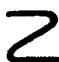
\includegraphics[keepaspectratio]{images/part001_587db9d1.jpg}}

\section{分次环的维数}

本节中，记 H 为一个具有正次数的 Z 型分次环，并以 \((\mathrm{H}_{n})_{n\in\mathbf{Z}}\) 表示其分次；因此有 \(H_{n}=\{0\}\)，当 n\textless0。

\subsection{与分次环关联的滤过环}

对于每个 \(n \in \mathbf{Z}\)，置 \(\mathrm{H}_{\geqslant n} = \sum_{i \geqslant n} \mathrm{H}_i\)。有 \(\mathrm{H} = \mathrm{H}_{\geqslant 0}\)；\(\mathrm{H}_{\geqslant n}\) 是 \(\mathrm{H}\) 的分次理想。令 S 为乘法子集 \(1 + \mathrm{H}_{\geqslant 1}\)，它由 H 中次数 0 分量等于 1 的元素组成，并考虑分式环 \(\mathrm{S}^{-1}\mathrm{H}\)。将 H 识别为其完备化 \(\hat{\mathrm{H}} = \prod_{n} \mathrm{H}_{n}\) 的一个子环（III, § 2, no. 12, 例 1）；由于 S 中的元素在 \(\hat{\mathrm{H}}\) 中可逆（III, § 2, no. 13, 引理 3），\(\mathrm{S}^{-1}\mathrm{H}\) 被识别为 \(\hat{\mathrm{H}}\) 的一个包含 H 的子环。对于 \(s \in \mathrm{S}\) 和 \(h \in \mathrm{H}_{\geqslant n}\)，\(s^{-1}h - h\) 中的元素 \(\hat{\mathrm{H}}\) 属于 \(\prod_{i \geqslant n} \mathrm{H}_i\)；因此有 \(\mathrm{S}^{-1}\mathrm{H}_{\geqslant n} = (\mathrm{S}^{-1}\mathrm{H}) \cap \prod_{i \geqslant n} \mathrm{H}_i\)。

由此得到：

命题 1. --- a) 理想 S \(^{-1}\) H \(_{≥n}\) 构成环 S \(^{-1}\) H 的一个穷尽且分离的滤过。

\begin{enumerate}
\def\labelenumi{\alph{enumi})}
\setcounter{enumi}{1}
\tightlist
\item
  从 H 到 \(S^{-1}H\) 的典范同态对每个 n 诱导出一个同构 \(u_{n}\)，它将 \(H_{n}\) 同构到 \(S^{-1}H_{\geqslant n}/S^{-1}H_{\geqslant n+1}\)；\(u_{n}\) 是从 H 到 \(S^{-1}H\) 的分次环同构的齐次分量，后者的滤过为 \(S^{-1}H_{\geqslant n}\)。
\end{enumerate}

注。--- 1) 若 \(h/s\) 是 \(\mathrm{S}^{-1}\mathrm{H}\) 中的元素，其中 \(h\in\mathrm{H}, s\in\mathrm{S}\)，则 h/s 可逆，当且仅当 h 的次数 0 分量在 \(h\)\(\mathrm{H}_{0}\) 中可逆。因此，若环 \(\mathrm{H}_{0}\) 是局部的，则环 \(\mathrm{S}^{-1}\mathrm{H}\) 是局部的，且典范嵌入 \(\mathrm{H}_{0}\to\mathrm{S}^{-1}\mathrm{H}\) 在剩余域上诱导出同构。

\begin{enumerate}
\def\labelenumi{\arabic{enumi})}
\setcounter{enumi}{1}
\tightlist
\item
  假设 H 由 \(H_{0}\) 和 \(H_{1}\) 生成；则对于每个 n，有 \(H_{n+1} = H_{1}.H_{n}\)，从而 \(H_{\geqslant n+1} = H_{1}.H_{\geqslant n}\)，以及 \(S^{-1}H_{\geqslant n+1} = H_{1}.S^{-1}H_{\geqslant n}\)。因此，\((S^{-1}H_{\geqslant n})\) 的滤过 \(S^{-1}H\) 是 \(S^{-1}H_{\geqslant 1}\)-进滤过。
\end{enumerate}

例子。--- 1) * 设 p 是 C{[}X₀, \ldots, Xₙ{]} 的一个分次素理想，且不同于由 Xᵢ 生成的理想；设 V 是 Pⁿ(C) 中由 p 定义的代数子簇，C 是 Cⁿ⁺¹ 中由 p 定义的代数子簇。则 C 是以 V 为底的锥，H = C{[}X₀, \ldots, Xₙ{]}/p 是 C 的仿射代数，而 S⁻¹H 是锥 C 在其顶点处的局部环。 *

\begin{enumerate}
\def\labelenumi{\arabic{enumi})}
\setcounter{enumi}{1}
\tightlist
\item
  设 A 是局部环，a 是 A 的理想且不同于 A。则 H = \(\bigoplus_{n} \mathfrak{a}^{n}/\mathfrak{a}^{n+1}\)
\end{enumerate}

是一个分次环，满足 \(H_{0} = A/\mathfrak{a}\) 是局部环；它由 \(H_{0}\) 和 \(H_{1}\) 生成。因此，环 \(S^{-1}H\) 是局部的，且滤过（ \(S^{-1}H_{\geq n}\) ）是 \(S^{-1}H_{\geq 1}\)-进滤过。注意，一般而言，环 A 与 \(S^{-1}H\) 并不同构。* 特别地，代数簇一般不在点的某个邻域内局部同构于它在该点的切锥。*

\subsection{分次理想的维数与链}

在本节中，记 dimgr(H) 为 H 的分次素理想链长度的上确界；同样，若 p 是 H 的分次素理想，记 htgr(p) 为 H 的、以 p 为最大元的分次素理想链长度的上确界。若 p 是分次素理想，则有 \(p \cap S = \varnothing\)；否则，p 将包含一个次数 0 分量等于 1 的元素，由于 p 是分次理想，遂包含 1。因而，从 H 的分次素理想集合到 \(p \mapsto S^{-1}p\) 的素理想集合的映射 \(S^{-1}H\) 是单射且递增的（II, § 2, no. 5, 命题 11）；因此，结合 § 1, no. 3 的命题 6 及命题 7 的推论，有：

命题 2. --- a) 有 \(\dim \mathrm{gr}(\mathrm{H}) \leqslant \dim (\mathrm{S}^{-1}\mathrm{H}) \leqslant \dim (\mathrm{H})\)。

\begin{enumerate}
\def\labelenumi{\alph{enumi})}
\setcounter{enumi}{1}
\tightlist
\item
  对于 H 的每个分次素理想 \(\mathfrak{p}\)，有 \(\operatorname{htgr}(\mathfrak{p}) \leqslant \operatorname{ht}(\mathrm{S}^{-1}\mathfrak{p}) = \operatorname{ht}(\mathfrak{p})\)。
\end{enumerate}

对于 H 的每个理想 a，记 \(a^{gr}\) 为包含于 a 的最大分次理想；有 \(a^{gr} = \sum_{n} (a \cap H_n)\)。

引理 1. --- a) 若 p 是 H 的素理想，则 \(\mathfrak{p}^{\mathrm{gr}}\) 是素理想。

\begin{enumerate}
\def\labelenumi{\alph{enumi})}
\setcounter{enumi}{1}
\item
  H 的分次理想集合中每个不同于 H 的极大元，都是包含 \(H_{\geq1}\) 的 H 的极大理想。
\item
  H 的每个极小素理想都是分次的。
\item
  这由 III, § 1, no. 4 的命题 4 得出。
\item
  设 m 是 H 的不同于 H 的分次理想。则有
\end{enumerate}

\[
\mathfrak {m} \subset (\mathfrak {m} \cap \mathrm{H} _ {0}) + \mathrm{H} _ {\geqslant 1} \neq \mathrm{H}.
\]

如果 m 是极大理想，则有 \(m = m_{0} + H_{\geq 1}\)，其中 \(m_{0}\) 是 \(H_{0}\) 的极大理想，从而得到 b)。

\begin{enumerate}
\def\labelenumi{\alph{enumi})}
\setcounter{enumi}{2}
\tightlist
\item
  设 p 是 H 的极小素理想。由于 \(p^{gr}\) 由 a) 知是素理想且包含于 p，故有 \(p = p^{gr}\)，从而得到 c)。
\end{enumerate}

引理 2.--- 设 p、q 是 H 的素理想，满足 q ⊂ p 且 q ≠ p。若 q \(^{gr}\) = p \(^{gr}\)，则 q 是分次的，p 不是分次的，且 ht(p/q) = 1。

注 1.--- 沿用第 1 号例 1 的记号。引理 2 表明：若 \(\mathbf{C}^{n+1}\) 中两个不可约子簇 Y、Z 具有相同的投影锥，且 \(Z \subset Y\)、\(Z \neq Y\)，则 Y 是 Z 的投影锥，而 Z 在 Y 中的余维数为 1。*

以 \(\mathrm{H} / \mathfrak{q}^{\mathrm{gr}}\) 替换 H，将问题化为 \(\mathfrak{q}^{\mathrm{gr}} = \{0\}\) 的情形。此时 H 是整环（引理 1, a)），\(\mathfrak{p}^{\mathrm{gr}} = 0\)，而要证明的是 \(\operatorname{ht}(\mathfrak{p}) \leqslant 1: this will indeed imply that  \operatorname{ht}(\mathfrak{q}) = 0\)，从而有 \(\mathfrak{q} = \{0\}\)。由于 \(\mathfrak{p}^{\mathrm{gr}} = \{0\}\)，对于每个 \(\mathfrak{p} \cap \mathrm{H}_n = \{0\}\)，有 \(n\)，且 \(\mathfrak{p}\) 与乘法子集 \(\mathrm{T} = \bigcup_{n} (\mathrm{H}_n - \{0\})\) 不相交。环 \(\mathrm{H}_{\mathfrak{p}}\) 因而同构于 \(\mathrm{T}^{-1}\mathrm{H}\) 的一个分式环，从而有

\[
\mathrm{ht} (\mathfrak {p}) = \dim (\mathrm{H} _ {\mathfrak {p}}) \leqslant \dim (\mathrm{T} ^ {- 1} \mathrm{H})
\]

（§ 1, no. 3, 命题 6 和命题 7）。但是，根据 V, § 1, no. 8 的引理 4，T \(^{-1}\) H 是域，或同构于环 K{[}X, X \(^{-1}\) {]}，其中 K 是域；因而有 dim(T \(^{-1}\) H) ≤ 1 及 ht(p) ≤ 1，这正是要证明的结论。

命题 3. --- 设 p 是 H 的素理想。若 p ≠ p \(^{gr}\)，则有 ht(p \(^{gr}\)) = ht(p) - 1。根据引理 1 a)，理想 p \(^{gr}\) 是素理想且包含于 p，故 ht(p \(^{gr}\)) ≤ ht(p) - 1。当 ht(p \(^{gr}\)) = +∞ 时命题显然，因此可设 ht(p \(^{gr}\)) \textless{} +∞。我们按 ht(p \(^{gr}\)) 归纳证明不等式 ht(p) ≤ ht(p \(^{gr}\)) + 1。只需证明：对于包含于 p 且不同于 p 的每个素理想 q，有 ht(q) ≤ ht(p \(^{gr}\))。按 q \(^{gr}\) ≠ p \(^{gr}\) 或 q \(^{gr}\) = p \(^{gr}\) 分两种情形。若 q \(^{gr}\) ≠ p \(^{gr}\)，则 ht(q \(^{gr}\)) \textless{} ht(p \(^{gr}\))；我们有

\[
\mathrm{ht} (\mathfrak {q}) \leqslant \mathrm{ht} (\mathfrak {q} ^ {\mathrm{gr}}) + 1,
\]

根据归纳假设（当 q ≠ q \(^{gr}\) 时）以及显然性（当 q = q \(^{gr}\) 时），我们得到 ht(q) ≤ ht(q \(^{gr}\)) + 1 ≤ ht(p \(^{gr}\))，这正是要证明的结论。若 q \(^{gr}\) = p \(^{gr}\)，则根据引理 2 有 q = q \(^{gr}\)，故 ht(q) = ht(q \(^{gr}\)) ≤ ht(p \(^{gr}\))，再次得到所需结论。

定理 1. --- 假设 H 是诺特环。

\begin{enumerate}
\def\labelenumi{\alph{enumi})}
\item
  H 的每条分次素理想链，若作为分次素理想链是饱和的，则作为素理想链也是饱和的。
\item
  对于 H 的每个分次素理想 p，有 htgr(p) = ht(S \(^{-1}\) p) = ht(p)。
\item
  我们有 \(\dim \mathrm{gr}(\mathbf{H}) = \dim (\mathbf{S}^{-1}\mathbf{H}) = \dim (\mathbf{H}).\)
\end{enumerate}

为证明 \(a\)，只需证明：若 \(\mathfrak{p}\) 和 \(\mathfrak{q}\) 是 H 的两个不同的分次素理想，满足 \(\mathfrak{q} \subset \mathfrak{p}\)，且 \(\mathfrak{q}\) 与 \(\mathfrak{p}\) 之间的每个分次素理想都等于 \(\mathfrak{p}\) 或 \(\mathfrak{q}\)，则 \(\mathrm{ht}(\mathfrak{p}/\mathfrak{q}) = 1\)。将 \(\mathfrak{q}\) 除去后，问题化为 \(\mathfrak{q} = \{0\}\) 的情形。因此还需证明：若 H 是整环，且 \(\mathfrak{p}\) 是 H 的一个理想，在不同于 \(\neq \{0\}\) 的分次素理想中为极小元，则有 \(\mathrm{ht}(\mathfrak{p}) = 1\)。现在设 \(a\) 是 \(\mathfrak{p}\) 中的非零齐次元素，令 r 为 H 的一个素理想，使得 \(a \in \mathfrak{r} \subset \mathfrak{p}\)，并且对于这些性质是极小的（II, § 2, no. 6, 引理 2）。由于 \(\mathfrak{r}^{\mathrm{gr}}\) 是素理想（引理 1，\(a\)），且非零，故有 \(\mathfrak{r}^{\mathrm{gr}} = \mathfrak{p}\)，从而 \(\mathfrak{p} = \mathfrak{r}\)。由于 H 是整环且为诺特环，\(\mathfrak{p}\) 的高度为 1（§ 3, no. 1, 命题 1），从而得到 \(a\)。

证明 b)。设 p 是 H 的一个分次素理想。有

\[
\operatorname{htgr} (\mathfrak {p}) \leqslant \operatorname{ht} \left(\mathrm{S} ^ {- 1} \mathfrak {p}\right) \leqslant \operatorname{ht} (\mathfrak {p})
\]

（命题 2）；我们按 ht(p) ≤ htgr(p) 归纳证明不等式。若 htgr(p) = 0，则 p 在分次素理想中是极小的，因而是极小的（引理 1，c)），且 ht(p) = 0。假设 htgr(p) \textgreater{} 0，并证明：对于每个包含于 p 且不同于 p 的素理想 q，有 ht(q) ≤ htgr(p) - 1。分两种情形。若 q 是分次的，则由归纳假设得出结论。若 q 不是分次的，则有 q \(^{gr}\) ≠ p，故根据归纳假设 ht(q \(^{gr}\) ) ≤ htgr(q \(^{gr}\) )，从而根据命题 3，ht(q) ≤ htgr(q \(^{gr}\) ) + 1；还需证明 htgr(q \(^{gr}\) ) ≤ htgr(p) - 2；但若 htgr(q \(^{gr}\) ) = htgr(p) - 1，则链 q \(^{gr}\) ⊂ p 根据 a) 将是饱和的，而这不可能，因为 q \(^{gr}\) ≠ q ≠ p。

最后证明 c)。有 dimgr(H) ≤ dim(S⁻¹H) ≤ dim(H)（命题 2），还需证明 dim(H) ≤ dimgr(H)，或等价地，对 H 的每个素理想 p，有 ht(p) ≤ dimgr(H)。于是设 p 是 H 的素理想。若 p 分次，则 ht(p) = htgr(p) ≤ dimgr(H)。若 p 非分次，则根据命题 3，有 ht(p) = htgr(p\(^{\mathrm{gr}}\)) + 1；令 m 为 H 中包含 p\(^{\mathrm{gr}}\) 的极大分次理想；根据引理 1 b)，m 是极大的，因而不同于 p\(^{\mathrm{gr}}\)，且有 htgr(p\(^{\mathrm{gr}}\)) + 1 ≤ htgr(m) ≤ dimgr(H)，从而再次有 ht(p) ≤ dimgr(H)。证明完毕。

注记 2. --- 存在非诺特的分次环 H，使 dimgr(H) \textless{} dim(H)（p.~99，练习 1）。

\subsection{分次模的维数}

在本节中，我们用 M 表示一个分次 H-模（Z 型）。

则 \(\mathbf{S}^{-1}\mathbf{M}\) 是一个 \(\mathbf{S}^{-1}\mathbf{H}\)-模；若置 \(\mathbf{M}_{\geqslant n} = \bigoplus_{i\geqslant n}\mathbf{M}_i\) ，则如

第 1 号中所述，集合序列 \(S^{-1}M_{\geqslant n}\) 是定义在

\(S^{-1}M\) 上的一个穷尽且分离的滤过；且典范映射 \(M \to S^{-1}M\) 诱导出从 M 到分次模 \(\oplus S^{-1}M_{\geqslant n}/S^{-1}M_{\geqslant n+1}\) 的一个同构。

引理 3. --- 假设 H 由 \(\mathbf{H}_{0} \cup \mathbf{H}_{1}\) 生成，而 M 由 \(\bigoplus_{i \leqslant n_{0}} \mathbf{M}_{i}\) 生成，其中 \(n_{0}\) 是适当的整数。则 \((\mathbf{S}^{-1}\mathbf{M}_{\geqslant n})\) 作为 \(\mathbf{S}^{-1}\mathbf{M}\) 的滤过，对于 \(\mathbf{S}^{-1}\mathbf{H}_{\geqslant 1}\) 的理想 \(\mathbf{S}^{-1}\mathbf{H}\) 是良好的。

当 \(n \geqslant n_0\) 时，\(\mathbf{M}_{\geqslant n+1} = \mathbf{H}_1 \cdot \mathbf{M}_{\geqslant n}\)，因而 \(\mathbf{S}^{-1} \mathbf{M}_{\geqslant n+1} = \mathbf{H}_1 \cdot \mathbf{S}^{-1} \mathbf{M}_{\geqslant n} = \mathbf{S}^{-1} \mathbf{H}_{\geqslant 1} \cdot \mathbf{S}^{-1} \mathbf{M}_{\geqslant n}\)。

命题 4. --- 假设 H 是诺特环且 M 是有限生成的。则 \(\dim_{\mathbf{H}}(\mathbf{M}) = \dim_{\mathbf{S}^{-1}\mathbf{H}}(\mathbf{S}^{-1}\mathbf{M})\)。

令 a 为 H-模 M 的湮灭子；它是 H 的一个分次理想。由于 M 是有限生成的 H-模，S \(^{-1}\) H-模 S \(^{-1}\) M 的湮灭子是 S \(^{-1}\) H 的理想 S \(^{-1}\) a。我们有 dim \(_{H}\) (M) = dim(H/a)，且 dim \(_{S^{-1}H}\) (S \(^{-1}\) M) = dim(S \(^{-1}\) H/S \(^{-1}\) a)。命题 4 由第 2 号的定理 1 c) 应用于分次环 H/a 即得。

命题 5. --- 假设 \(\mathbf{H}_{0}\) 是局部阿廷环，\(\mathbf{H}\) 由 \(\mathbf{H}_{0} \cup \mathbf{H}_{1}\) 生成，\(\mathbf{H}_{1}\) 是有限型的 \(\mathbf{H}_{0}\)-模，而 \(\mathbf{M}\) 是非零的有限型 \(\mathbf{H}\)-模。则对于每个 \(\mathbf{M}_{n}\)，\(\mathbf{H}_{0}\) 都是有限生成的 \(n\)-模，具有有限长度且非零；并且存在 \(\mathbf{Q}(\mathbf{T}) \in \mathbf{Z}[\mathbf{T}, \mathbf{T}^{-1}]\)，使得 \(\mathbf{Q}(1) > 0\)，且在环 \(\mathbf{Z}((\mathbf{T}))\) 中有

\[
\sum_ {n \in \mathbf {Z}} \mathrm{long} _ {\mathrm{H} _ {0}} (\mathrm{M} _ {n}). \mathrm{T} ^ {n} = (1 - \mathrm{T}) ^ {- d}. \mathrm{Q} (\mathrm{T}),
\]

其中 \(d = \dim_{\mathbf{H}}(\mathbf{M})\)。

环 \(\mathbf{S}^{-1}\mathbf{H}\) 是局部诺特环（第 1 号，注 1）；\(\mathbf{S}^{-1}\mathbf{H}\)-模 \(\mathbf{S}^{-1}\mathbf{M}\) 是非零有限型模，并且其维数为 \(d = \dim_{\mathbf{H}}(\mathbf{M})\)（命题 4）。此外，\(\mathbf{S}^{-1}\mathbf{H}_{\geqslant 1}\) 是 \(\mathbf{S}^{-1}\mathbf{H}\) 的一个定义理想（§ 3，第 2 号，引理 2），而 \(\mathbf{S}^{-1}\mathbf{M}_{\geqslant n}\) 是 \(\mathbf{S}^{-1}\mathbf{H}_{\geqslant 1}\) 上关于 \(\mathbf{S}^{-1}\mathbf{M}\) 的良好滤过（引理 3）。最后，等式 \(_{\mathbf{S}^{-1}\mathbf{H}}\mathbf{S}^{-1}\mathbf{M}_{\geqslant n}/\mathbf{S}^{-1}\mathbf{M}_{\geqslant n+1} = \text{long}_{\mathbf{H}_0}(\mathbf{M}_n)\) 对每个 \(n\) 成立。因此只需应用第 § 4 节（第 3 号和第 4 号）的定理 2 和定理 3。

注。--- 除了确定整数 d 之外，命题 5 直接由第 § 4 节第 2 号的定理 1 得出。

推论。--- 设 A 是诺特局部环，q 是 A 的一个定义理想。则有 \(\dim(A) = \dim(\text{gr}_{\mathfrak{q}}(A))\)。

将命题 5 应用于 M = H = gr\_q(A) 的情形，得到关系

\[
\sum_ {n \geqslant 0} \mathrm{long} _ {\mathrm{A} / \mathfrak {q}} (\mathfrak {q} ^ {n} / \mathfrak {q} ^ {n + 1}). \mathrm{T} ^ {n} = (1 - \mathrm{T}) ^ {- d} \mathrm{Q} (\mathrm{T})
\]

其中 \(d = \dim(\mathrm{gr}_{\mathfrak{q}}(\mathbf{A}))\) 且 \(\mathbf{Q}(1) \neq 0\)。根据第 § 4 节第 4 号的定理 3，有 \(d = \dim(\mathbf{A})\)，故推论得证。

命题 6. --- 假设 \(\mathbf{H}_{0}\) 是局部阿廷环，\(\mathbf{H}\) 是有限型的 \(\mathbf{H}_{0}\)-代数，而 \(\mathbf{M}\) 是有限型的 \(\mathbf{H}\)-模。

\begin{enumerate}
\def\labelenumi{\alph{enumi})}
\item
  设 \(a_1, \ldots, a_n\) 是 H 中的元素，均为次数 \(> 0\) 的齐次元素；令 \(\varphi\) 为一个（\(\mathbf{H}_0\)-代数）同态，它从 \(\mathbf{H}_0[\mathbf{X}_1, \ldots, \mathbf{X}_n]\) 到 H，并将 \(\mathbf{X}_i\) 送到 \(a_i\)，其中 \(1 \leqslant i \leqslant n\)。则 \(S^{-1}H\)-模 \(S^{-1}M / \sum_{i=1}^{n}(a_i/1) \cdot S^{-1}M\) 具有有限长度，当且仅当 \(\varphi_*(M)\) 是 \(\mathbf{H}_0[\mathbf{X}_1, \ldots, \mathbf{X}_n]\) 上的有限生成模。
\item
  存在一个 H 中元素的族 \((a_{1},...,a_{d})\)，它们都是同一次数 \textgreater0 的齐次元素，其中 \(d=\dim_{\mathrm{H}}(\mathbf{M})\)，并且 \((a_{1}/1,...,a_{d}/1)\) 是 \(S^{-1}H\)-模 \(S^{-1}M\) 的一个极大正割序列。若进一步，H 由 \(H_{1}\) 生成（作为 \(H_{0}\)-代数），且 \(H_{0}\) 的剩余域是无限的，则可取次数为 1 的 \(a_{i}\)。
\item
  置 \(\mathbf{N} = \mathbf{M} / \sum_{i=1}^{n} a_i \mathbf{M}\)。根据命题 4，有 \(\dim_{\mathrm{H}}(\mathbf{N}) = \dim_{\mathrm{S}^{-1}\mathrm{H}}(\mathrm{S}^{-1}\mathrm{N})\)。因此，\(\mathrm{S}^{-1}\mathrm{H}\)-模 \(\mathrm{S}^{-1}\mathrm{N}\) 具有有限长度，当且仅当 H-模 N 具有有限长度；也就是说，当且仅当 N 是有限型的 \(\mathrm{H}_0\)-模。若 \(\varphi_*(\mathbf{M})\) 是定义在 \(\mathrm{H}_0[\mathrm{X}_1, ..., \mathrm{X}_n]\) 上的、通过同态 \(\varphi : \mathrm{H}_0[\mathrm{X}_1, ..., \mathrm{X}_n] \to \mathbf{H}\) 从 M 导出的模，则有 \(\mathbf{N} = \varphi_*(\mathbf{M}) / \sum_{i=1}^{n} X_i \cdot \varphi_*(\mathbf{M})\)。因此（A, II, p.~171，推论 3 和注），\(\varphi_*(\mathbf{M})\) 是 \(\mathrm{H}_0[\mathrm{X}_1, ..., \mathrm{X}_n]\) 上的有限生成模，当且仅当 N 是有限型的 \(\mathrm{H}_0\)-模。这就证明了 a)。
\end{enumerate}

为证明 b)，我们先建立一个引理。

引理 4. --- 设 \(b\) 是 H 中一个次数 \(>0\) 的齐次元素，并且不属于任何极小元 \(\mathfrak{p}\)，这里的极小元取自 \(\operatorname{Supp}(\mathbf{M})\) 且满足 \(\dim(\mathrm{H}/\mathfrak{p}) = \dim_{\mathrm{H}}(\mathbf{M})\)。则 \(\dim_{\mathrm{H}}(\mathbf{M}/b\mathbf{M}) = \dim_{\mathrm{H}}(\mathbf{M}) - 1\)。

置 \(d = \dim_{\mathbf{H}}(\mathbf{M})\)。根据 \(b\) 的定义，有 \(\dim_{\mathbf{H}}(\mathbf{M}/b\mathbf{M}) < d\)。根据命题 4，有

\[
\dim_ {\mathrm{H}} (\mathrm{M} / b \mathrm{M}) = \dim_ {\mathrm{S} ^ {- 1} \mathrm{H}} \left(\mathrm{S} ^ {- 1} \mathrm{M} / (b / 1). \mathrm{S} ^ {- 1} \mathrm{M}\right)
\]

最后，有

\[
\dim_ {\mathrm{S} ^ {- 1} \mathrm{H}} (\mathrm{S} ^ {- 1} \mathrm{M} / (b / 1). \mathrm{S} ^ {- 1} \mathrm{M}) \geqslant \dim_ {\mathrm{S} ^ {- 1} \mathrm{H}} (\mathrm{S} ^ {- 1} \mathrm{M}) - 1.
\]

最后，有

\[
\dim_ {S ^ {- 1} H} (S ^ {- 1} M) = \dim_ {H} (M) = d
\]

因此 \(\dim_{\mathrm{H}}(\mathrm{M}/b\mathrm{M}) \geqslant d - 1\)，从而引理 4 得证。

我们继续证明命题 6 b)。可设 \(\dim_{\mathbf{H}}(\mathbf{M}) > 0\)。注意，\(\operatorname{Supp}(\mathbf{M})\) 的每个极小元都是分次的（将第 2 号的引理 1 应用于 H 除以 M 的湮灭子所得的商）。根据 III, § 1, 第 4 号的命题 8，存在 H 的一个齐次元素 \(b\)，次数为 \(>0\)，且不属于任何极小元 \(\mathfrak{p}\)；这些极小元取自 \(\operatorname{Supp}(\mathbf{M})\)，并满足 \(\dim(\mathrm{H}/\mathfrak{p}) = \dim_{\mathbf{H}}(\mathbf{M})\)。根据引理 4，有 \(\dim_{\mathbf{H}}(\mathbf{M}/b\mathbf{M}) = \dim_{\mathbf{H}}(\mathbf{M}) - 1\)。再假设 H 由 \(\mathrm{H}_{1}\) 生成（作为 \(\mathrm{H}_{0}\)-代数），且剩余域 \(k\) 是 \(\mathrm{H}_{0}\) 的无限域。对于每个满足以下条件的极小元 \(\mathfrak{p}\)：它属于 \(\operatorname{Supp}(\mathbf{M})\)，且满足 \(\dim(\mathrm{H}/\mathfrak{p}) = \dim_{\mathbf{H}}(\mathbf{M})\)，考虑向量子空间 \(\mathrm{V}_{\mathfrak{p}} = (\mathfrak{p} \cap \mathrm{H}_{1}) \otimes_{\mathrm{H}_{0}} k\)，它是 \(k\)-向量空间 \(\mathrm{V} = \mathrm{H}_{1} \otimes_{\mathrm{H}_{0}} k\) 的子空间。若有 \(\mathrm{V}_{\mathfrak{p}} = \mathrm{V}\)，则有 \(\mathfrak{p} \cap \mathrm{H}_1 = \mathrm{H}_1\)（II, §3, 第 2 号，命题 4），从而 \(\mathrm{H}_1 \subset \mathfrak{p}\)，且 \(\dim_{\mathrm{H}}(\mathbf{M}) = \dim(\mathrm{H}/\mathfrak{p}) \leqslant \dim(\mathrm{H}/\mathrm{H}_{\geqslant 1}) = 0\)，这与假设不符。由于假设 \(k\) 是无限的，各个 \(\mathrm{V}_{\mathfrak{p}}\) 的并集不同于 V；若 \(b \in \mathrm{H}_1\) 且 \(b \otimes 1\) 不属于其中任何一个 \(\mathrm{V}_{\mathfrak{p}}\)，则 \(\dim(\mathrm{M}/b\mathrm{M}) = \dim_{\mathrm{H}}(\mathrm{M}) - 1\)。

对 \(d = \dim_{\mathbf{H}}(\mathbf{M})\) 作归纳，便可构造 H 中元素的序列 \((b_1, \ldots, b_d)\)，其中 \(b_i\) 是次数 \(n_i > 0\) 的齐次元素，并且 \(\mathbf{M} / \sum_{i=1}^{n} b_i \mathbf{M}\) 是有限长度的 H-模。若假设 H 由 \(\mathbf{H}_1\) 生成（作为 \(\mathbf{H}_0\)-代数），且 \(\mathbf{H}_0\) 的剩余域是无限的，则可设 \(n_i = 1\)，其中 \(i = 1, \ldots, d\)。根据命题 4，有 \(\dim_{\mathbf{S}^{-1}\mathbf{H}}(\mathbf{S}^{-1}\mathbf{M}) = d\)，并且

\[
\dim_ {\mathrm{S} ^ {- 1} \mathrm{H}} (\mathrm{S} ^ {- 1} \mathrm{M} / \sum_ {i = 1} ^ {d} (b _ {i} / 1). \mathrm{S} ^ {- 1} \mathrm{M}) = 0.
\]

于是 \((b_{1} / 1,\dots,b_{d} / 1)\) 是 \(\mathbf{S}^{-1}\mathbf{H}\)-模 \(\mathbf{S}^{-1}\mathbf{M}\) 的一个极大正割序列。置 \(a_{i} = b_{i}^{(n_{1}\dots n_{d}) / n_{i}}\)，其中 \(1\leqslant i\leqslant d\)；则 \(a_{i}\) 具有相同的次数，并且 \((a_{1} / 1,\dots,a_{d} / 1)\) 是 \(\mathbf{S}^{-1}\mathbf{M}\) 的一个极大正割序列（§ 3，第 2 号，注 3）。

推论 1. --- 假设 \(\mathbf{H}_0\) 是一个域，且 \(\mathbf{H}\) 是有限型的 \(\mathbf{H}_0\)-代数。置 \(n = \dim(\mathbf{H})\)。存在齐次元素 \(a_1, ..., a_n\)，它们属于 \(\mathbf{H}\)，且都具有 \(>0\) 的同一次数，使 \(\mathbf{H}_0\)-同态 \(\varphi: \mathbf{H}_0[\mathbf{X}_1, ..., \mathbf{X}_n] \to \mathbf{H}\)（由 \(\varphi(\mathbf{X}_i) = a_i\)，\(i = 1, ..., n\) 定义）是单射，并使 \(\mathbf{H}\) 成为有限的 \(\mathbf{H}_0[\mathbf{X}_1, ..., \mathbf{X}_n]\)-代数。若 \(\mathbf{H}\) 由 \(\mathbf{H}_1\) 生成（作为 \(\mathbf{H}_0\)-代数），且 \(\mathbf{H}_0\) 是无限的，则可取次数为 1 的 \(a_i\)。

根据命题 6，存在一个上述形式的 \(\mathbf{H}_0\)-同态 \(\varphi\)，使 H 成为 \(\mathbf{H}_0[\mathbf{X}_1, \ldots, \mathbf{X}_n]\)-有限代数。根据第 § 2 节第 3 号的定理 1，有

\[
\dim \left(\mathrm{H} _ {0} \left[ \mathrm{X} _ {1}, \dots , \mathrm{X} _ {n} \right] / (\operatorname{Ker} \varphi)\right) = \dim (\mathrm{H});
\]

因为有

\[
\dim (\mathrm{H}) = n = \dim \left(\mathrm{H} _ {0} \left[ \mathrm{X} _ {1}, \dots , \mathrm{X} _ {n} \right]\right),
\]

且 \(\mathrm{H}_0[\mathrm{X}_1, \dots, \mathrm{X}_n]\) 是整环，这就推出 \(\operatorname{Ker} \varphi = \{0\}\)。

注。--- 设 \((h_{1}, \ldots, h_{r})\) 是 \(H_{0}\)-向量空间 \(H_{1}\) 的一个有限生成系。对于 \(\lambda = (\lambda_{1}, \ldots, \lambda_{r}) \in H_{0}^{r}\)，置 \(h_{\lambda} = \lambda_{1} h_{1} + \cdots + \lambda_{r} h_{r}\)。命题 6 和推论 1 的证明给出如下结果：由 \((\lambda_{1}, \ldots, \lambda_{n})\) 组成的、属于 \((\mathrm{H}_{0}^{r})^{n}\) 且使元素 \(a_{i} = h_{\lambda_{i}} \in H_{1}\) 满足推论 1 结论的元素集合，包含 \((\mathrm{H}_{0}^{r})^{n}\) 中有限个不等于整个空间的向量子空间之并的补集。

推论 2. --- 设 A 是诺特局部环且 \(n\in\mathbb{N}\)。要有 \(\dim(\mathbf{A})\geqslant n\)，充要条件是对于每个整数 \(r\geqslant0\)，有

\[
\left[ \mathfrak {m} _ {\mathrm{A}} ^ {r} / \mathfrak {m} _ {\mathrm{A}} ^ {r + 1}: \kappa_ {\mathrm{A}} \right] \geqslant \binom {n + r - 1} {n - 1}, \quad \left(\text { resp.   long } _ {\mathrm{A}} (\mathrm{A} / \mathfrak {m} _ {\mathrm{A}} ^ {r + 1}) \geqslant \binom {n + r} {n}\right);
\]

对于每个 r 都取等号，当且仅当 A 是维数为 n 的正则环。

该条件是充分的（§ 4，第 4 号，定理 3 以及 § 5，第 2 号，定理 1）。下面证明其必要性。考虑分次环 gr(A) = gr \(_{m_A}\) (A)；令 k 为 κ \(_A\) 的一个无限扩域，并置 H = k ⊗ κ \(_A\) gr(A)。环 H 的维数 ≥ n（命题 5 及其推论）；因此由推论 1，得到分次 k-代数的一个单射分次同态 φ : H \(_0\) {[}X \(_1\) , \ldots, X \(_n\) {]} → H。于是，对于每个整数 r ≥ 0，有

\[
\left[ \mathrm{gr} _ {r} (\mathrm{A}): \kappa_ {\mathrm{A}} \right] = \left[ \mathrm{H} _ {r}: \mathrm{H} _ {0} \right] \geqslant \binom {n + r - 1} {n - 1},
\]

且每个 \(r\) 都取等号会推出 \(\varphi\) 为双射，从而 A 正则（ \(\S\) 5，第 2 号，定理 1）。

等式

\[
\mathrm{long} _ {\mathbf {A}} (\mathrm{A} / \mathfrak {m} _ {\mathbf {A}} ^ {r + 1}) = \sum_ {i = 0} ^ {r} \left[ \mathrm{gr} _ {i} (\mathbf {A}): \kappa_ {\mathbf {A}} \right]
\]

以及

\[
\binom {n + r} {n} = \sum_ {i = 0} ^ {r} \binom {n + i - 1} {n - 1}
\]

从而得到关于函数 \(r \mapsto \text{long}_{\mathbf{A}}(\mathbf{A}/m_{\mathbf{A}}^{r+1})\) 的相应断言。

\subsection{维数的半连续性}

引理 5.--- 设 A 是一个环，r 是其根基，\(\mathbf{R} = \bigoplus_{i \in \mathbf{Z}} \mathbf{R}_i\) 是一个分次 A-代数，\(\mathbf{M} = \bigoplus_{i \in \mathbf{Z}} \mathbf{M}_i\) 是一个分次 R-模。假设每个 \(\mathbf{M}_i\) 都是有限型的 A-模

并且 M/rM 是有限生成的 R/rR-模。则 M 是有限生成的 R-模。设 \(m_{1}, \ldots, m_{n}\) 是 M 中的齐次元素，它们在 M/rM 中的像生成 R/rR-模 M/rM。令 N 为由 \(\{m_{1}, \ldots, m_{n}\}\) 生成的 M 的（分次）子 R-模。对于每个 \(i \in \mathbf{Z}\)，有 \(M_{i} = N_{i} + rM_{i}\)，因而 \(M_{i} = N_{i}\)（II, §3, 第 2 号，命题 4）；故 M = N。

引理 6. --- 设 \(\rho: \mathbf{B} \to \mathbf{C}\) 是环同态，S 是 B 的一个乘法子集。假设 C 是有限生成的 B-代数，且 \(\mathbf{S}^{-1}\mathbf{C}\) 是有限的 \(\mathbf{S}^{-1}\mathbf{B}\)-代数。则存在 \(f \in \mathbf{S}\)，使得 \(\mathbf{C}_f\) 是有限的 \(\mathbf{B}_f\)-代数。

设 X 是 B-代数 C 的一个有限生成集。对于每个 \(x \in X\)，x 在 \(S^{-1}C\) 中的像在 \(S^{-1}B\) 上整，因此存在整数 \(n(x) \geqslant 0\)、元素 \(b_{1}(x), \ldots, b_{n(x)}(x) \in B\) 以及元素 \(f(x) \in S\)，使得

\[
f (x) x ^ {n (x)} + b _ {1} (x) x ^ {n (x) - 1} + \dots + b _ {n (x)} = 0.
\]

置 \(f = \prod_{x \in X} f(x)\)；对于每个 \(x\)，\(X\) 中的该元素在 \(C_f\) 中的像都在 \(B_f\) 上整，故 \(C_f\) 是有限的 \(B_f\)-代数（V, § 1, 第 1 号，命题 4）。

命题 7. — 假设 H 是有限型的 \(H_{0}\)-代数。则函数 \(\mathfrak{p} \mapsto \dim(\mathrm{H} \otimes_{\mathrm{H}_{0}} \kappa(\mathfrak{p}))\) 在 \(\operatorname{Spec}(\mathrm{H}_{0})\) 上是上半连续的。

由于 H 作为 \(H_{0}\)-代数是有限生成的，每个 \(H_{i}\) 都是有限生成的 \(H_{0}\)-模（III, § 1, 第 2 号，命题 1 的推论），并且 H 作为 \(H_{0}\)-代数由 \(H_{0} \oplus H_{1} \oplus \cdots \oplus H_{r}\) 生成，其中 \(r \geqslant 0\) 是适当的整数。取 \(\mathfrak{p} \in \operatorname{Spec}(H_{0})\)，置 \(\dim(H \otimes_{H_{0}} \kappa(\mathfrak{p})) = n \geqslant 0\)。根据命题 6 的推论 1，存在 H 中的元素 \(a_{1}, ..., a_{n}\)，它们都是同一次数 \(d > 0\) 的齐次元素，使得 \(\kappa(\mathfrak{p})\)-同态 \(\overline{\varphi}: \kappa(\mathfrak{p})[X_{1}, ..., X_{n}] \to H \otimes_{H_{0}} \kappa(\mathfrak{p})\) 将 \(X_{i}\) 送到 \(a_{i} \otimes 1\)（\(1 \leqslant i \leqslant n\)），并使 \(H \otimes_{H_{0}} \kappa(\mathfrak{p})\) 成为有限的 \(\kappa(\mathfrak{p})[X_{1}, ..., X_{n}]\)-代数。令 \(\varphi\) 为一个 \(H_{0}\)-同态，它从 \(H_{0}[X_{1}, ..., X_{n}] = R\) 到 H，并将 \(X_{i}\) 送到 \(a_{i}\)，其中 \(1 \leqslant i \leqslant n\)。若对每个 \(m \in \mathbf{Z}\) 置 \(H_{m}' = \sum_{(m-1)d < i \leqslant md} H_{i}\)，则在 H 上得到一个 \(\mathbf{Z}\)-型分次，且与由 \(\varphi\) 给出的 R-模结构相容。每个 \(H_{m}'\) 都是有限型的 \(H_{0}\)-模。根据引理 5，\(H_{\mathfrak{p}}\) 是有限生成的 \(R_{\mathfrak{p}}\)-模。根据引理 6，存在 \(f \in H_{0} - \mathfrak{p}\)，使得 \(H_{f}\) 是有限型的 \(R_{f}\)-模。对于每个 \(\mathfrak{q} \in \operatorname{Spec}(H_{0})_{f}\)，\(H \otimes_{H_{0}} \kappa(\mathfrak{q})\) 是有限的 \(\kappa(\mathfrak{q})[X_{1}, ..., X_{n}]\)-代数，故 \(\dim(H \otimes_{H_{0}} \kappa(\mathfrak{q})) \leqslant n\)（\S 2，第 3 号，定理 1），这就完成了证明。

注记。--- 1) * 在代数几何中，命题 7 蕴含：代数簇之间的射影态射的纤维维数是上半连续的。 *

\begin{enumerate}
\def\labelenumi{\arabic{enumi})}
\setcounter{enumi}{1}
\tightlist
\item
  我们稍后将看到，若 \(\rho:A\to B\) 是环同态，使 \(B\) 成为有限型的 \(A\)-代数，则函数 \(\mathfrak{q}\mapsto\dim_{\mathfrak{q}}(B\otimes_{A}\kappa(\rho^{-1}(q)))\) 在 \(\operatorname{Spec}(B)\) 上是上半连续的（参见 p. 101，练习 10）。
\end{enumerate}

\subsection{分次正则代数}

在本节中，假设 \(H_{0}\) 是一个域，且 H 是有限型的 \(H_{0}\)-代数。

置 \(H_{+} = H_{\geqslant 1}\)；它是 H 的一个极大理想。环 \(S^{-1}H\) 可识别为 H 的局部环 \(H_{H_{+}}\)，对应于理想 \(H_{+}\)；其极大理想是 \((\mathrm{H}_{+})_{\mathrm{H}_{+}} = \mathrm{S}^{-1}\mathrm{H}_{+}\)，其剩余域可识别为 \(H_{0}\)。

命题 8. --- a) 有 \(\dim(\mathbf{H}) \leqslant [\mathbf{H}_{+}/\mathbf{H}_{+}^{2}:\mathbf{H}_{0}]\)。

\begin{enumerate}
\def\labelenumi{\alph{enumi})}
\setcounter{enumi}{1}
\tightlist
\item
  以下条件等价：
\end{enumerate}

\begin{enumerate}
\def\labelenumi{(\roman{enumi})}
\item
  \(\dim (\mathrm{H}) = [\mathrm{H}_{+} / \mathrm{H}_{+}^{2}:\mathrm{H}_{0}]\) ;
\item
  诺特局部环 \(\mathbf{S}^{-1}\mathbf{H}\) 是正则的；
\item
  H 作为 \(H_{0}\)-代数由一族次数 \textgreater{} 0 的、在 \(H_{0}\) 上代数无关的齐次元素生成。
\end{enumerate}

\begin{enumerate}
\def\labelenumi{\alph{enumi})}
\setcounter{enumi}{2}
\tightlist
\item
  假设 b) 的条件成立，并令 \(a_{1}, \ldots, a_{n} \in \mathbf{H}\) 是次数 \textgreater{} 0 的齐次元素。以下条件等价：
\end{enumerate}

\begin{enumerate}
\def\labelenumi{(\roman{enumi})}
\item
  \(a_{i}\) 的类构成 \(\mathbf{H}_{0}\)-向量空间 \(\mathbf{H}_{+}/\mathbf{H}_{+}^{2}\) 的一个基；
\item
  \(a_{i}/1\) 构成正则诺特局部环 \(\mathbf{S}^{-1}\mathbf{H}\) 的一个坐标系；
\item
  \(a_{i}\) 在 \(\mathbf{H}_{0}\) 上代数无关，并生成 \(\mathbf{H}\)（作为 \(\mathbf{H}_{0}\)-代数）。
\end{enumerate}

我们有 \(\dim(\mathbf{H})=\dim(\mathbf{S}^{-1}\mathbf{H})\)（第 2 号，定理 1），并且 \([\mathbf{H}_{+}/\mathbf{H}_{+}^{2}:\mathbf{H}_{0}]=[(\mathbf{S}^{-1}\mathbf{H}_{+})/(\mathbf{S}^{-1}\mathbf{H}_{+})^{2}:\mathbf{H}_{0}]\)（II, § 3, 第 3 号，命题 9）；根据 § 5，第 1 号，这推出 \(a\) 以及等价关系 (i) \(\Leftrightarrow\) (ii)（分别在 \(b\) 和 \(c\) 中）。其中的两个蕴含 (iii) \(\Rightarrow\) (i) 分别位于 \(b\) 和 \(c\) 中，显然成立。现证明蕴含 (i) \(\Rightarrow\) (iii)。因此，假设 \(\dim(\mathbf{H})=[\mathbf{H}_{+}/\mathbf{H}_{+}^{2}:\mathbf{H}_{0}]\)，并令齐次元素 \(a_{1},\ldots,a_{n}\) 属于 H，次数为 \(>0\)，且它们的类构成 \(\mathbf{H}_{+}/\mathbf{H}_{+}^{2}\) 的一个基；考虑分次代数同态 \(\varphi:\mathrm{H}_{0}[\mathrm{X}_{1},\ldots,\mathrm{X}_{n}]\to\mathrm{H}\)，它将 \(\mathrm{X}_{i}\) 送到 \(a_{i}\)。H 的理想 \(\mathrm{H}_{+}\) 由 \(a_{i}\) 生成（A, II, p.~171, 推论 2 和注）；因此同态 \(\varphi\) 是满射（III, § 1, 第 2 号，命题 1）。但是，有

\[
\dim \left(\mathrm{H} _ {0} \left[ \mathrm{X} _ {1}, \dots , \mathrm{X} _ {n} \right]\right) = n = \dim (\mathrm{H}) = \dim \left(\mathrm{H} _ {0} \left[ \mathrm{X} _ {1}, \dots , \mathrm{X} _ {n} \right] / (\operatorname{Ker} \varphi)\right)
\]

（§ 2，第 4 号，定理 3 的推论 1），因此 Ker φ = 0，因为 H₀{[}X₁, \ldots, Xₙ{]} 是整环。这就证明了断言 (iii)。

在 \(b\) ) 的假设下，称 H 为正则的 \(\mathrm{H}_{0}\)-分次代数，或 \(\mathrm{H}_{0}\)-分次多项式代数。在 \(c\) ) 的假设下，称 \(a_{i}\) 构成 H 的一个分次坐标系。

注记。--- 1) 采用 \(c\) ) 的记号，令 \(d_{i}\) 为 \(a_{i}\) 的次数（ \(1 \leqslant i \leqslant n\) ）。则庞加莱级数 \(\mathbf{P}_{\mathrm{H}} = \sum_{n \in \mathbf{Z}} [\mathrm{H}_{n} : \mathrm{H}_{0}] \cdot \mathrm{T}^{n}\) 等于 \(\prod_{i} (1 - \mathrm{T}^{d_{i}})^{-1}\)（§4，第 2 号，例 1）。因此，若 H 是 \(\mathrm{H}_{0}\)-分次多项式代数，则有

\[
\mathrm{P} _ {\mathrm{H}} = \prod_ {n} (1 - \mathrm{T} ^ {n}) ^ {- \delta (n)}, \quad \text { with } \quad \delta (n) = \left[ (\mathrm{H} _ {+} / \mathrm{H} _ {+} ^ {2}) _ {n}: \mathrm{H} _ {0} \right].
\]

\begin{enumerate}
\def\labelenumi{\arabic{enumi})}
\setcounter{enumi}{1}
\tightlist
\item
  反之，存在整数 \(d_{i}>0\) 使 \(\mathbf{P}_{\mathbf{H}}=\prod_{i}(1-\mathbf{T}^{d_{i}})^{-1}\)，并不意味着 H 是分次多项式代数；例如，若 H 由一个次数为 1 的元素 X 和一个次数为 2 的元素 Y 生成，且唯一关系为 \(\mathbf{X}^{2}=0\)，则有 \(\mathbf{P}_{\mathbf{H}}=(1-\mathbf{T})^{-1}\)。
\end{enumerate}

\section{重数}

在本段中，约定 A 表示一个诺特环。

\subsection{模关于理想的重数}

设 M 是有限生成的 A-模，q 是 A 的一个理想，包含于 A 的根基中，且 M/qM 具有有限长度。假设 M 不为 0，置 \(d = \dim_{\mathbf{A}}(\mathbf{M})\)。根据第 § 4 节第 3 号定理 2 的推论及第 4 号注 2，存在唯一的整数 \(e_{\mathfrak{q}}(\mathbf{M}) > 0\)，使得对于每个整数 \(n \geqslant 1\)

\[
\operatorname{long} _ {\mathbf {A}} (\mathrm{M} / \mathfrak {q} ^ {n + 1} \mathrm{M}) = e _ {\mathfrak {q}} (\mathrm{M}) \frac {n ^ {d}}{d !} + \beta_ {n} n ^ {d - 1}
\]

其中 \(\beta_{n}\) 在 \(n\) 无限增大时趋于一个极限。

定义 1. --- 整数 \(e_{\mathfrak{q}}(\mathbf{M})\) 称为 A-模 \(\mathbf{M}\) 关于理想 q 的重数。

当需要指明环 A 时，也记作 \(e_{\mathfrak{q}}^{\mathbf{A}}(\mathbf{M})\)。当 A 是极大理想为 m 的局部环时，分别用 \(e(\mathbf{M})\) 或 \(e^{\mathbf{A}}(\mathbf{M})\) 表示 \(e_{\mathfrak{m}}(\mathbf{M})\) 或 \(e_{\mathfrak{m}}^{\mathbf{A}}(\mathbf{M})\)。

注记。--- 1) 若 q' 是 A 的一个理想，包含于 A 的根基中且包含 q，则 \(e_{\mathfrak{q}'}(\mathbf{M}) \leqslant e_{\mathfrak{q}}(\mathbf{M})\)；并且，若 M 的 \(q'\)-进滤过是 q-良好的，则有 \(e_{\mathfrak{q}'}(\mathbf{M}) = e_{\mathfrak{q}}(\mathbf{M})\)（§ 4，第 3 号，定理 2）。

\begin{enumerate}
\def\labelenumi{\arabic{enumi})}
\setcounter{enumi}{1}
\item
  若 M 具有有限长度，则有 \(e_{\mathfrak{q}}(\mathbf{M}) = \mathrm{long}_{\mathbf{A}}(\mathbf{M})\)（§ 4，第 3 号，注 3）。
\item
  若 \(d > 0\)，则有
\end{enumerate}

\[
\operatorname{long} _ {\mathrm{A} / \mathfrak {q}} (\mathfrak {q} ^ {n} \mathrm{M} / \mathfrak {q} ^ {n + 1} \mathrm{M}) = e _ {\mathfrak {q}} (\mathrm{M}) \frac {n ^ {d - 1}}{(d - 1) !} + \alpha_ {n} n ^ {d - 2}
\]

其中 \(\alpha_{n}\) 在 \(n\) 无限增大时趋于一个极限（§ 4，第 3 号，定理 2 的推论）。

\begin{enumerate}
\def\labelenumi{\arabic{enumi})}
\setcounter{enumi}{3}
\tightlist
\item
  由于根据 § 4，第 4 号定理 3 的推论，有
\end{enumerate}

\[
e _ {\mathrm{q}} (\mathbf {M}) = \sum e _ {\mathrm{q} _ {\mathrm{m}}} (\mathbf {M} _ {\mathrm{m}})
\]

求和遍历 A 的所有极大理想 m，其中满足

\[
\mathfrak {m} \in \operatorname{Supp} (\mathbf {M}) \cap \mathrm{V} (\mathfrak {q}) \quad \text { and } \quad \dim_ {\mathrm{A} _ {\mathfrak {m}}} (\mathrm{M} _ {\mathfrak {m}}) = d  .
\]

由注记 2 和 3 可知，\(e_{\mathfrak{q}}(\mathbf{M})\) 只取决于分次 A/q-模 \(\mathrm{gr}_{\mathfrak{q}}(\mathbf{M})\)。因此：

命题 1.--- 设 \(\hat{\mathbf{A}}\) 和 \(\hat{\mathbf{M}}\) 分别是 \(\mathbf{A}\) 和 \(\mathbf{M}\) 关于 q-进拓扑的完备化；则 \(e_{\mathfrak{q}}^{\mathbf{A}}(\mathbf{M}) = e_{\mathfrak{q}\hat{\mathbf{A}}}^{\hat{\mathbf{A}}}(\hat{\mathbf{M}})\)。

命题 2. --- 假设 A 是正则局部环（§ 5，第 1 号，定义 1）；则 e(A) = 1。

这由 § 5 第 2 号的定理 1 得出。

注记 5. --- 即使 A 不正则，也可能有 \(e(A) = 1\)（p.~104，练习 5）。事实上，诺特局部环 A 正则，当且仅当 \(\hat{A}\) 是整环且有 \(e(A) = 1\)（p.~108，练习 24）。

例。--- 根据定义，有 \(e_{\mathfrak{q}^{r}}(\mathbf{M}) = r^{d}e_{\mathfrak{q}}(\mathbf{M})\)，其中 \(d = \dim_{\mathbf{A}}(\mathbf{M})\)。因此，若 A 是正则局部环，则 \(e_{\mathfrak{m}_{\mathbf{A}}^{r}}(\mathbf{A}) = r^{d}\)。例如，若 A 是离散赋值环，则 \(e_{\mathfrak{q}}(\mathbf{A}) = \text{long}(\mathbf{A}/\mathfrak{q})\)。

设 q 是 A 的一个理想，包含于 A 的根基中，令 \(\mathcal{C}(\mathfrak{q})\) 为满足 \(M/qM\) 具有有限长度的有限生成 A-模的同构类集合。对于每个 \(d \in \mathbf{N}\)，以 \(\mathcal{C}(\mathfrak{q})_{\leq d}\) 表示 \(\mathcal{C}(\mathfrak{q})\) 中由维数 \(\leqslant d\) 的 A-模的同构类组成的部分。定义映射 \(e_{\mathfrak{q},d}: \mathcal{C}(\mathfrak{q})_{\leq d} \to \mathbf{Z}\)：规定 \(e_{\mathfrak{q},d}(\mathbf{M}) = e_{\mathfrak{q}}(\mathbf{M})\)（当 \(\dim(\mathbf{M}) = d\) 时），否则 \(e_{\mathfrak{q},d}(\mathbf{M}) = 0\)。根据第 § 4 节第 3 号的命题 5，这个映射是可加的；由此（A, VIII, § 10, 第 2 号）得到一个仍记作 \(e_{\mathfrak{q},d}\) 的同态，它从 Grothendieck 群 \(K(\mathcal{C}(\mathfrak{q})_{\leq d})\) 到 \(\mathbf{Z}\)，并且在 \(K(\mathcal{C}(\mathfrak{q})_{\leq d-1})\) 上为零。仿照 § 1 第 5 号的论证，得到：

命题 3. — 设 \(\mathbf{M}\) 是有限生成的 A-模，维数 \(d \geqslant 0\)。令 \(\Phi\) 为由极小元 \(\mathfrak{p}\) 构成的集合，这些极小元属于 \(\operatorname{Supp}(\mathbf{M})\) 且满足 \(\dim(\mathbf{A}/\mathfrak{p}) = d\)。设 \(\mathfrak{q}\) 是 A 的一个理想，包含于 A 的根基中，且 \(\mathbf{M}/\mathfrak{q}\mathbf{M}\) 具有有限长度。则有

\[
e _ {\mathfrak {q}} (\mathrm{M}) = \sum_ {\mathfrak {p} \in \Phi} \operatorname{long} _ {\mathrm{A} _ {\mathfrak {p}}} (\mathrm{M} _ {\mathfrak {p}}) \cdot e _ {\mathfrak {q}} (\mathrm{A} / \mathfrak {p}).
\]

推论。— 假设 A 是半局部环，且 q 是 A 的一个定义理想。

\begin{enumerate}
\def\labelenumi{\alph{enumi})}
\item
  有 \(e_{\mathfrak{q}}(\mathbf{A}) = \sum_{\mathfrak{p}} e_{\mathfrak{q}}(\mathbf{A}/\mathfrak{p})\)，其中 \(\mathfrak{p}\) 遍历 \(\mathbf{A}\) 的极小素理想中满足 \(\dim(\mathbf{A}/\mathfrak{p}) = \dim(\mathbf{A})\) 的那些理想。
\item
  假设 A 是整环，且 M 是有限生成的 A-模，满足 \(\dim_{\mathbf{A}}(\mathbf{M}) = \dim(\mathbf{A})\)。则有 \(e_{\mathfrak{q}}(\mathbf{M}) = \operatorname{rg}(\mathbf{M}) \cdot e_{\mathfrak{q}}(\mathbf{A})\)。
\end{enumerate}

\subsection{重数与平坦扩张}

命题 4. — 设 \(\rho: A \to B\) 是诺特局部环之间的局部同态，且 \(N\) 是一个 \(B\)-模，在 \(A\) 上平坦，并且 \(N \otimes_A \kappa_A\) 是有限长度的 \(B\)-模。若 \(M\) 是一个非零有限生成的 \(A\)-模，且 q 是 \(A\) 的一个不同于 \(A\) 的理想，并且 \(M/qM\) 具有有限长度，则 \((M \otimes_A N)/(qB)(M \otimes_A N)\) 是一个非零有限生成的 \(B\)-模，具有有限长度，并且有

\[
e _ {\mathrm{qB}} ^ {\mathrm{B}} (\mathbf {M} \otimes_ {\mathrm{A}} \mathbf {N}) = \operatorname{long} _ {\mathrm{B}} (\mathbf {N} \otimes_ {\mathrm{A}} \kappa_ {\mathrm{A}}). e _ {\mathrm{q}} ^ {\mathrm{A}} (\mathbf {M}).
\]

设 L 是一个有限长度为 r 的 A-模。则 L 有一个长度为 r 的 Jordan–Hölder 序列，其商同构于 \(\kappa_{A}\)；由于 N 在 A 上平坦，B-模 \(L \otimes_{A} N\) 有一个长度为 r 的合成序列，其商同构于 \(N \otimes_{A} \kappa_{A}\)，因而其长度为 \(r \cdot \operatorname{long}_{\mathbf{B}}(\mathbf{N} \otimes_{\mathbf{A}} \kappa_{\mathbf{A}})\)。由于 B-模 \((\mathbf{M} \otimes_{\mathbf{A}} \mathbf{N})/(\mathbf{q}\mathbf{B})^{n}(\mathbf{M} \otimes_{\mathbf{A}} \mathbf{N})\) 同构于 \((\mathbf{M}/\mathbf{q}^{n}\mathbf{M}) \otimes_{\mathbf{A}} \mathbf{N}\)，且这一同构对每个 \(n \in \mathbf{N}\) 都成立，根据重数的定义，命题得证。

推论。— 假设 B 在 A 上平坦，且 \(\rho(\mathfrak{m}_{\mathbf{A}})\) B = \(\mathfrak{m}_{\mathbf{B}}\)。则

\[
e _ {\mathbf {q B}} ^ {\mathbf {B}} (\mathbf {M} \otimes_ {\mathbf {A}} \mathbf {B}) = e _ {\mathbf {q}} ^ {\mathbf {A}} (\mathbf {M}).
\]

这特别适用于 B 是 A 关于一个不同于 A 的理想的完备化 * 或 Hensel 化 *，或 A 的一个膨胀 *（例如 A 的严格 Hensel 化）时。 *

例。— * 设 X 是复代数簇，\(\mathcal{O}_{X,x}\) 是 X 在有理点 \(x\) 处的局部环，\(X^{an}\) 是与 X 关联的解析空间；仍以 \(x\) 表示 \(X^{an}\) 中对应于前述 \(x\) 的点，并令 \(\mathcal{O}_{X^{an},x}\) 为 \(X^{an}\) 在 \(x\) 处的局部环。则 \(e(\mathcal{O}_{X^{an},x}) = e(\mathcal{O}_{X,x})\)。 *

\subsection{重数与有限扩张}

命题 5. — 假设 A 是半局部环，且 \(\rho: A \to B\) 是使 B 成为有限生成 A-模的环同态。设 N 是一个非零有限生成的 B-模，q 是 A 的一个理想，包含于 A 的根基中，并且 N/qN 具有有限长度。在 B 的极大理想中，将满足条件的那些记为 \(\mathfrak{m}_1, \ldots, \mathfrak{m}_r\)，其中 \(\dim_{\mathrm{B}_{\mathfrak{m}_i}} (\mathrm{N}_{\mathfrak{m}_i}) = \dim_{\mathrm{B}} (\mathrm{N})\)（根据 IV, § 2, 第 5 号，命题 9 的推论 3，它们的数目有限）。置 \(\mathbf{B}_i = \mathbf{B}_{\mathfrak{m}_i}\)，\(\mathfrak{q}_i = \mathfrak{q}\mathbf{B}_i\)，其中 \(1 \leqslant i \leqslant r\)。则有以下等式

\[
\dim_ {A} (N) = \dim_ {B} (N),
\]

\[
e _ {\mathfrak {q} \mathrm{B}} ^ {\mathbf {B}} (\mathbf {N}) = \sum_ {i = 1} ^ {r} e _ {\mathfrak {q} _ {i}} ^ {\mathbf {B} _ {i}} (\mathbf {N} _ {\mathfrak {m} _ {i}}),
\]

\[
e _ {\mathfrak {q}} ^ {\mathrm{A}} (\mathrm{N}) = \sum_ {i = 1} ^ {r} \left[ \mathrm{B} / \mathfrak {m} _ {i}: \mathrm{A} / \rho^ {- 1} (\mathfrak {m} _ {i}) \right] e _ {\mathfrak {q} _ {i}} ^ {\mathrm{B} _ {i}} (\mathrm{N} _ {\mathfrak {m} _ {i}}).
\]

第一个等式由 § 2，第 3 号，定理 1 c) 得出；第二个等式由第 1 号的注记 4 得出（注意，m \(_{i}\) 属于 V(qB)（\(1 \leqslant i \leqslant r\)），因为根据 V, § 2，第 1 号，命题 1，有 \(\rho^{-1}(m_{i}) \supset q\)）。下面证明第三个等式。设 E 是一个有限长度的 B-模；有

\[
\operatorname{long} _ {\mathbf {A}} (\mathbf {E}) = \sum_ {m} \left[ \mathrm{B} / m: \mathrm{A} / \rho^ {- 1} (m) \right]. \operatorname{long} _ {\mathrm{B} _ {m}} \left(\mathrm{E} _ {m}\right),
\]

m 遍历 B 的极大理想集合；当 E 是某个 B/m 时，这一点确实显然；一般情形由此得到，因为 E 有一个合成序列，其商同构于 B/m。将这个公式应用于 B-模 N/q \(^{n+1}\) N，便根据重数的定义得到所需等式。

推论。— 若对于所有 i 都有 \(\left[\mathrm{B}/\mathfrak{m}_{i}:\mathrm{A}/\rho^{-1}(\mathfrak{m}_{i})\right]=1\)，则有 \(e_{\mathfrak{q}}^{\mathrm{A}}(\mathrm{N})=e_{\mathfrak{q}\mathrm{B}}^{\mathrm{B}}(\mathrm{N})\)。

引理 1. — 设 \(\rho: A \to B\) 是环同态，且 \(\mathfrak{p}\) 是 A 的一个素理想。考虑以下两个性质：

\begin{enumerate}
\def\labelenumi{(\roman{enumi})}
\item
  典范同态 \(\tilde{\rho}\) 从 \(\mathbf{A}_{\mathfrak{p}}\) 到 \(\mathbf{A}_{\mathfrak{p}} \otimes_{\mathbf{A}} \mathbf{B}\) 是双射；
\item
  存在 B 中唯一的素理想 \(\mathfrak{r}\)，它位于 \(\mathfrak{p}\) 之上，且典范同态 \(\rho_{\mathfrak{p}}\) 从 \(A_{\mathfrak{p}}\) 到 \(B_{\mathfrak{r}}\) 是双射。
\end{enumerate}

我们有 \((\mathrm{i}) \Rightarrow (\mathrm{ii})\)。若 \(\mathfrak{p}\) 是极小的，或者 \(\mathbf{B}\) 整于 \(\mathbf{A}\)，则有 \((\mathrm{i}) \Leftrightarrow (\mathrm{ii})^{1}\)。

环 \(\mathbf{A}_{\mathfrak{p}} \otimes_{\mathbf{A}} \mathbf{B}\) 可识别为 B 的分式环 \(S^{-1} \mathbf{B}\)，其中乘法子集 \(S = \rho(A - \mathfrak{p})\) 是 B 的子集。因而 \(S^{-1} \mathbf{B}\) 的素理想正是 \(S^{-1} \mathfrak{q}\)，其中 \(\mathfrak{q}\) 是满足 \(\rho^{-1}(\mathfrak{q}) \subset \mathfrak{p}\) 的 B 的素理想；若 \(\mathfrak{q}\) 是这样的理想，则 \((S^{-1} \mathbf{B})_{S^{-1} \mathfrak{q}}\) 可识别为 \(\mathbf{B}_{\mathfrak{q}}\)（II, § 2, 第 5 号，命题 11）。

若性质 (i) 成立，则存在（V, § 2，第 1 号，引理 1）中所述的 B 中唯一的素理想 \(\mathfrak{r}\)，满足 \(\rho^{-1}(\mathfrak{r}) = \mathfrak{p}\)。此外，\(B_{\mathfrak{r}}\) 可识别为分式环 \((S^{-1}B)_{S^{-1}\mathfrak{r}}\)，因而也可识别为 \((A_{\mathfrak{p}})_{s}\)，其中 \(s\) 是 \(S^{-1}\mathfrak{r}\) 在同构 \(\tilde{\rho}: A_{\mathfrak{p}} \to S^{-1}B\) 下的逆像；并且 \(\tilde{\rho}^{-1}(S^{-1}\mathfrak{r}) = (A - \mathfrak{p})^{-1}\mathfrak{p} = \mathfrak{p}A_{\mathfrak{p}}\)，从而有 (ii)。

反之，若 (ii) 成立，令 r 为位于 p 之上的 B 的唯一素理想。由于 \((\mathrm{S}^{-1}\mathrm{B})_{\mathrm{S}^{-1}\mathrm{r}}\) 可识别为 \(B_{r}\)，只需证明 \(S^{-1}B\) 是以 \(S^{-1}r\) 为极大理想的局部环；也就是说，B 的每个满足 \(\rho^{-1}(q) \subset p\) 的素理想 q 都包含于 r。若 p 是极小的，则有 \(\rho^{-1}(q) = p\)，故 q = r。若 B 整于 A，则根据 V, § 2，第 1 号，定理 1 的推论 2，存在 B 的一个素理想 \(r'\)，使 \(q \subset r'\) 且 \(\rho^{-1}(r') = p\)；必有 \(r' = r\)，故 \(q \subset r\)。

引理 2.--- 假设 A 是半局部环；设 q 是 A 的一个定义理想，且 \(\rho : A \to B\) 是使 B 成为有限生成 A-模的环同态。假设，对于 A 的每个素理想 \(\mathfrak{p}\)（必为极小的），若满足 \(\dim(A/\mathfrak{p}) = \dim(A)\)，则存在 B 中唯一的素理想 \(\mathfrak{r}\)，位于 \(\mathfrak{p}\) 之上，且典范同态 \(\rho_{\mathfrak{p}} : A_{\mathfrak{p}} \to B_{\mathfrak{r}}\) 是双射。则有 \(\dim_{A}(B) = \dim(A)\) 且 \(e_{\mathfrak{q}}^{A}(B) = e_{\mathfrak{q}}^{A}(A)\)。记 \(\mathfrak{S}_{A}\)（分别为 \(\mathfrak{S}_{B}\)）为如下集合：A 的素理想 \(\mathfrak{p}\) 满足

\[
\dim (\mathrm{A} / \mathfrak {p}) = \dim (\mathrm{A}) (\text { resp. } \dim_ {\mathrm{A}} (\mathrm{B} / \mathfrak {p} \mathrm{B}) = \dim_ {\mathrm{A}} (\mathrm{B}));
\]

我们有 \(\mathfrak{S}_{\mathbf{A}} \neq \emptyset\)。取 \(\mathfrak{p} \in \mathfrak{S}_{\mathbf{A}}\)；由假设，存在一个位于 \(\mathfrak{p}\) 之上的 B 的素理想。于是 \(\rho^{-1}(\mathfrak{pB}) = \mathfrak{p}\)（II, § 2, 第 5 号，命题 11 的推论 3），并且

\[
\dim (\mathrm{A} / \mathfrak {p}) = \dim (\mathrm{B} / \mathfrak {p B}) = \dim_ {\mathrm{A}} (\mathrm{B} / \mathfrak {p B})
\]

根据 § 2，第 3 号，定理 1 b) 和 c)，因此有

\[
\dim_ {\mathrm{A}} (\mathrm{B}) \geqslant \dim_ {\mathrm{A}} (\mathrm{B} / \mathfrak {p B}) = \dim (\mathrm{A} / \mathfrak {p}) = \dim (\mathrm{A}) \geqslant \dim_ {\mathrm{A}} (\mathrm{B}).
\]

这说明 \(\mathfrak{S}_{\mathrm{A}} \subset \mathfrak{S}_{\mathrm{B}}\) 且 \(\dim(\mathrm{A}) = \dim_{\mathrm{A}}(\mathrm{B})\)。反之，若 \(\mathfrak{p} \in \mathfrak{S}_{\mathrm{B}}\)，则有不等式

\[
\dim_ {A} (B / p B) = \dim_ {A} (B) = \dim (A) \geqslant \dim (A / p) \geqslant \dim_ {A} (B / p B),
\]

从而 \(p \in \mathfrak{S}_A\)，且 \(\mathfrak{S}_B = \mathfrak{S}_A\)。根据第 1 号的命题 3 及其推论，有

\[
e _ {\mathfrak {q}} ^ {\mathrm{A}} (\mathrm{A}) = \sum_ {\mathfrak {p} \in \mathfrak {S} _ {\mathrm{A}}} e _ {\mathfrak {q}} ^ {\mathrm{A}} (\mathrm{A} / \mathfrak {p}) \quad \text { and } \quad e _ {\mathfrak {q}} ^ {\mathrm{A}} (\mathrm{B}) = \sum_ {\mathfrak {p} \in \mathfrak {S} _ {\mathrm{B}}} \operatorname{long} _ {\mathrm{A} _ {\mathfrak {p}}} (\mathrm{A} _ {\mathfrak {p}} \otimes_ {\mathrm{A}} \mathrm{B}) e _ {\mathfrak {q}} ^ {\mathrm{A}} (\mathrm{A} / \mathfrak {p});
\]

根据引理 1，有 \(\operatorname{long}_{A_{\mathfrak{p}}}(A_{\mathfrak{p}} \otimes_{A} B) = 1\)，其中 \(\mathfrak{p} \in \mathfrak{S}_{A}\)；从而 \(e_{\mathfrak{q}}^{A}(A) = e_{\mathfrak{q}}^{A}(B)\)。

命题 6. --- 假设 A 是半局部且约化的；设 q 是 A 的一个定义理想；设 A' 是 A 的全分式环，B 是 A' 的一个有限 A-子代数。则 B 是半局部的，且 qB 是它的一个定义理想。假设，对于 B 的每个满足 \(\dim(\mathbf{B}_{\mathfrak{m}})=\dim(\mathbf{B})\) 的极大理想 m，都有 \([\mathbf{B}/\mathfrak{m}:\mathbf{A}/(\mathbf{A}\cap\mathfrak{m})]=1\)。则有 \(e_{\mathfrak{q}}^{\mathbf{A}}(\mathbf{A})=e_{\mathfrak{q}\mathbf{B}}^{\mathbf{B}}(\mathbf{B})\)。

根据 IV, § 2，第 5 号，命题 9 的推论 3，B 是半局部的，定义理想为 qB。根据命题 5 的推论，有 \(e_{qB}^{B}(B) = e_{q}^{A}(B)\)。由于 A' 可识别为 \(\prod_{p} A_p\)，其中 p 遍历 A 的极小素理想集合（IV, § 2，第 5 号，命题 10），故对于 A 的每个极小素理想 p，典范映射 \(A_{p} \to A_{p} \otimes_{A} B\) 都是双射。于是由引理 1 和引理 2，\(e_{q}^{A}(B) = e_{q}^{A}(A)\)，从而命题得证。

例。--- 设 \(k\) 是特征 \(\neq 2\) 的域，取 A 为局部环 \(k[[X, Y]]/(X^{2} + Y^{2})\)，其剩余域为 \(k\)。取 \(B = k[[X, T]]/(T^{2} + 1)\)，其中 \(T = Y/X\)。分两种情形：若 -1 是元素 \(i\)（来自 \(k\)）的平方，则 B 有两个极大理想，分别由 \(\{X, T + i\}\) 和 \(\{X, T - i\}\) 生成；它们的剩余域为 \(k\)，并且有 \(e_{\mathfrak{m}_{A}}^{A}(A) = e_{\mathfrak{m}_{A}B}^{B}(B) = 2\)。若 -1 不是 \(k\) 中的平方，则 B 有唯一极大理想 (X)，其剩余域为 \(k[T]/(T^{2} + 1)\)，且有 \(e_{\mathfrak{m}_{A}}^{A}(A) = 2\)，\(e_{\mathfrak{m}_{A}B}^{B}(B) = 1\)。

\subsection{重数与正割序列}

命题 7. --- 假设 A 是局部环。设 s 是一个整数 ≥ 1，并且对于 \(1 \leqslant i \leqslant s\)，令 \(\delta_{i}\) 是 \textgreater{} 0 的整数，\(x_{i}\) 是 \(m_{A}^{\delta_{i}}\) 中的元素，\(\xi_{i}\) 是它在 \(m_{A}^{\delta_{i}}/m_{A}^{\delta_{i}+1}\) 中的类。假设 \((x_{1}, \ldots, x_{s})\) 是 A 的一个正割序列。令 x 表示由 \((x_{1}, \ldots, x_{s})\) 生成的 A 的理想。则有 \(e(A/x) \geqslant \delta_{1} \ldots \delta_{s} \cdot e(A)\)，当 \((\xi_{1}, \ldots, \xi_{s})\) 是 gr(A) 中的完全正割序列时取等号。

置 B = A/x，考虑形式级数

\[
\mathrm{H} _ {\mathrm{A}} = \sum_ {n \geqslant 0} \operatorname{long} (\mathfrak {m} _ {\mathrm{A}} ^ {n} / \mathfrak {m} _ {\mathrm{A}} ^ {n + 1}). \mathrm{T} ^ {n}, \quad \mathrm{H} _ {\mathrm{B}} = \sum_ {n \geqslant 0} \operatorname{long} (\mathfrak {m} _ {\mathrm{B}} ^ {n} / \mathfrak {m} _ {\mathrm{B}} ^ {n + 1}). \mathrm{T} ^ {n}
\]

并且 \(\mathrm{H}_{\mathrm{B}}^{(s)} = (1 - \mathrm{T})^{-s}\mathrm{H}_{\mathrm{B}}\)。根据第 § 4 节第 5 号的命题 6，在 \(\mathbf{Z}[[T]]\) 中有不等式

\[
\mathrm{H} _ {\mathrm{B}} ^ {(s)} \geqslant \left(\prod_ {i = 1} ^ {s} \frac {1 - \mathrm{T} ^ {\delta_ {i}}}{1 - \mathrm{T}}\right) \mathrm{H} _ {\mathrm{A}},
\]

当序列 \((\xi_{1}, \ldots, \xi_{s})\) 是完全正割序列时取等号。但是

\[
\mathrm{R(T)} = \prod_ {i = 1} ^ {s} \frac {1 - \mathrm{T} ^ {\delta_ {i}}}{1 - \mathrm{T}}
\]

这是 \(\mathbf{Z}[\mathrm{T}]\) 中的一个多项式，且 \(\mathbf{R}(1) = \delta_1 \ldots \delta_s\)。置 \(\dim(\mathbf{A}) = d\)；有 \(\dim(\mathbf{B}) = d - s\)。根据第 §4 节第 3 号的定理 2，存在 \(\mathbf{R}_{\mathbf{A}}\) 和 \(\mathbf{R}_{\mathbf{B}}\)，它们属于 \(\mathbf{Z}[\mathrm{T}, \mathrm{T}^{-1}]\)，使得

\[
\mathrm{H} _ {\mathrm{A}} = (1 - \mathrm{T}) ^ {- d} \mathrm{R} _ {\mathrm{A}} (\mathrm{T}), \quad \mathrm{R} _ {\mathrm{A}} (1) = e (\mathrm{A}),
\]

\[
\mathrm{H} _ {\mathrm{B}} = (1 - \mathrm{T}) ^ {- d + s} \mathrm{R} _ {\mathrm{B}} (\mathrm{T}), \quad \mathrm{R} _ {\mathrm{B}} (1) = e (\mathrm{A} / x).
\]

因此有

\[
(1 - \mathrm{T}) ^ {- d} \mathrm{R} _ {\mathrm{B}} (\mathrm{T}) = \mathrm{H} _ {\mathrm{B}} ^ {(s)} \geqslant \left(\prod_ {i = 1} ^ {s} \frac {1 - \mathrm{T} ^ {\delta_ {i}}}{1 - \mathrm{T}}\right) \mathrm{H} _ {\mathrm{A}} = (1 - \mathrm{T}) ^ {- d} \mathrm{R} (\mathrm{T}) \mathrm{R} _ {\mathrm{A}} (\mathrm{T}),
\]

并且当序列 \((\xi_{1},\ldots,\xi_{s})\) 是完全正割序列时取等号。根据第 § 4 节第 1 号的引理 2，结论得出。

注记。--- 反之，可以证明（参见 p. 103，练习 4），若 A 是正则的且 \(e(\mathrm{A}/\mathfrak{x})=\delta_{1}\ldots\delta_{s}\)，则序列 \((\xi_{1},\ldots,\xi_{s})\) 是完全正割序列。

例。--- 设 A 是形式幂级数环 \(k[[X_1, ..., X_n]]\)，定义在域 \(k\) 上；设 \(F_1, ..., F_s\) 是 A 的元素，令 \(\mathfrak{a}\) 为它们生成的理想，并置 \(B = A/\mathfrak{a}\)。将 \(P_1, ..., P_s \in k[X_1, ..., X_n]\) 记为级数 \(F_1, ..., F_s\) 的初始形式，并令 \(\delta_1, ..., \delta_s\) 为它们各自的次数。若序列 \(F_1, ..., F_s\) 在 A 中是正割的，则有 \(e(B) \geqslant \delta_1 ... \delta_s\)；若序列 \(P_1, ..., P_s\) 在环 \(k[X_1, ..., X_n]\) 中是完全正割的，则有 \(e(B) = \delta_1 ... \delta_s\)。

例如，考虑环 \(\mathbf{B} = k[[\mathrm{X},\mathrm{Y}]] / \mathfrak{a}\)，其中 \(\mathfrak{a}\) 由 \(\mathrm{X}^2 + \mathrm{Y}^3\) 和 \(\mathrm{X}^2 + \mathrm{Y}^4\) 生成；由上述不等式得 \(e(\mathbf{B})\geqslant 4\)；注意到 \(\mathfrak{a}\) 也由元素 \(\mathrm{X}^2 + \mathrm{Y}^3\) 和 \(\mathrm{Y}^4 -\mathrm{Y}^3\) 生成，而这些元素的初始形式序列是完全正割的，故得到 \(e(\mathbf{B}) = 6\)。
